\chapter{Special Theory of Relativity}
The $20^{\text{th }}$ century saw essentially two major triumphs in physics: the discovery of quantum mechanics and the discovery of relativity.
\section{Reference Frame}
\begin{wrapfigure}{r}{0.40\textwidth}
	\begin{center}
		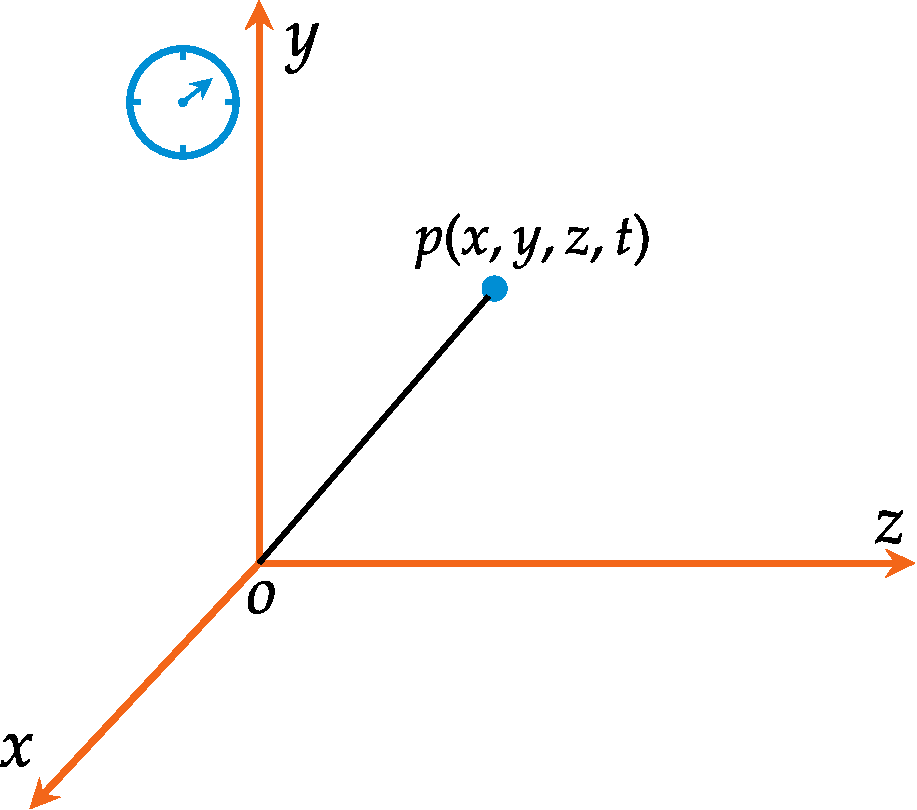
\includegraphics[width=0.25\textwidth]{str1}
	\end{center}
	\caption{Reference Frame}
\end{wrapfigure}
Reference frames are physico-mathematical structures that have the purpose of allowing the objective description, also from a quantitative viewpoint, of physical phenomena that are observed in nature.\\
In order to describe the motion of a particle in space, we need to know its position at different instants of time. This needs the choice of reference body or coordinate system. If we imagine a coordinate system attached to a rigid body and we describe the position of any particle relative to it, then such a coordinate system is called frame of reference. For the location of the objects, the position vectors are drawn from the origin $O$ of the coordinate system . \textbf{A reference frame with four coordinates $\mathrm{x}, \mathrm{y}, \mathrm{z}, \mathrm{t}$ is referred as space-time frame}. The simplest frame of reference is a cartesian coordinate system. 
\subsection{Inertial Frame of Reference}
Inertial frames are frames in which Newton's laws of motion holds true.
It is the one in which the law of inertia holds true i.e., if a particle, subject to no external force, is found to move in a straight line with constant velocity (or to remain at rest), then the coordinate system used for this purpose is called inertial frame.
\begin{align*}
\intertext{We know that according to  Newton's second law of motion,}
F&=\frac{dP}{dt}\\
&=\frac{d(mV)}{dt}
\intertext{If\ $F=0$}
\frac{dV}{dt}&=0
\intertext{Then velocity is constant in inertial frame of reference.}
\end{align*}
Inertial frames are  related by a constant velocity along any axis.  An object is at rest in an inertial frame when it's position in space does not change with time.\\
 
\subsection{Non-Inertial Frame of Reference}
 Accelerated frame of reference in which Newton's law does not hold good.\\\\
 If there is an observer  in a rotating frame then, according to the obeserver a person standing out of his  frame is seems to be accelerating , and then,  according to the observer ,  a force seems to be acting on the person. Then , first law of motion will not be holding in an accelerated frame.
\section{Galilean Transformation } 
An event or physical phenomena, observed simultaneously in two separate reference frames, will have to separate set of coordinates. \textbf{Equation relating two coordinate system  is called transformation equation.} \\
Let $ S $ and $ S^{\prime} $ be two inertial frame of reference with observer at origin $\mathrm{O}$ and $\mathrm{O}^{\prime}$ moving with a relative velocity $y$ along positive direction of $x$.
The Galilean transformation successfully explained the invariance of laws of Newtonian mechanics in different inertial frame. Let the coordinates $(x, t)$ denote the location of an event in the non moving frame $s$ and $\left(x^{\prime}, t^{\prime}\right)$ denote the location of the same event in the moving frame $s^{\prime}$. The Galilean transformation which relates the two coordinate systems is:
\begin{align*}
	x^{\prime} &=x-v t \\
	y^{\prime} &=y \\
	z^{\prime} &=z \\
	t^{\prime} &=t
\end{align*}
\subsubsection{Inverse transformation}
\begin{align*}
	x&=x^{\prime}+v t^{\prime}\\  y&=y^{\prime} \\z&=z^{\prime} \\
	t&=t^{\prime}
\end{align*}
\subsubsection{Velocity transformation}
\begin{align*}
	u_{x}^{\prime}&=u_{x}-v \\u_{y}^{\prime}&=u_{y}\\ u_{z}^{\prime}&=u_{z}
	\intertext { \textbf{Inverse Velocity Transformation }}
	u_{x}&=u_{x}^{\prime}+v \\ u_{y}&=u_{y}^{\prime} \\ u_{z}&=u_{z}^{\prime}
\end{align*}
\subsubsection{Transformation of acceleration}
Let $ a $ and  ${a}^{\prime}$  be the acceleration in ${S}$ and ${S}^{\prime}$ frame of reference.\\
We have, 
\begin{align*}
a^{\prime}&=\frac{d u^{\prime}}{d t}\\&=\frac{d(u-v)}{d t}\hspace{3cm} [\because v=0]\\&=\frac{d u}{d t}-0\\&=a\\
\intertext{$\therefore$ Acceleration is invariant under Galilean transformation.}
\end{align*}
\section{Postulates of Special Theory of Relativity}
Einstein in 1905 , formulated this special theory of relativity on the basis of following postulates:
\begin{enumerate}
	\item \textbf{The laws of physics are same in all inertial frames. This is the principle of relativity.}
	\item \textbf{The speed of light in vacuum is constant and same as observed from all inertial frames. This is known as the principle of constant of speed of light.}
\end{enumerate}

The first postulate implies that not only the laws of mechanics but also that of electrodynamics and optics should be same for all inertial reference systems. There is no privileged frame like ether or absolute space.\\\\
 If Einstein's postulate that the velocity of light is the same in all inertial frames  is correct, then the Galilean transformation is not the correct way to transform space-time coordinates between two inertial frames.einstein showed that, Maxwell's theory is consistent with special relativity whereas, Newtonian mechanics is not, and his modification of these branches of physics into accord.
 \section{Lorentz transformation}
\begin{figure}[H]
	\centering
	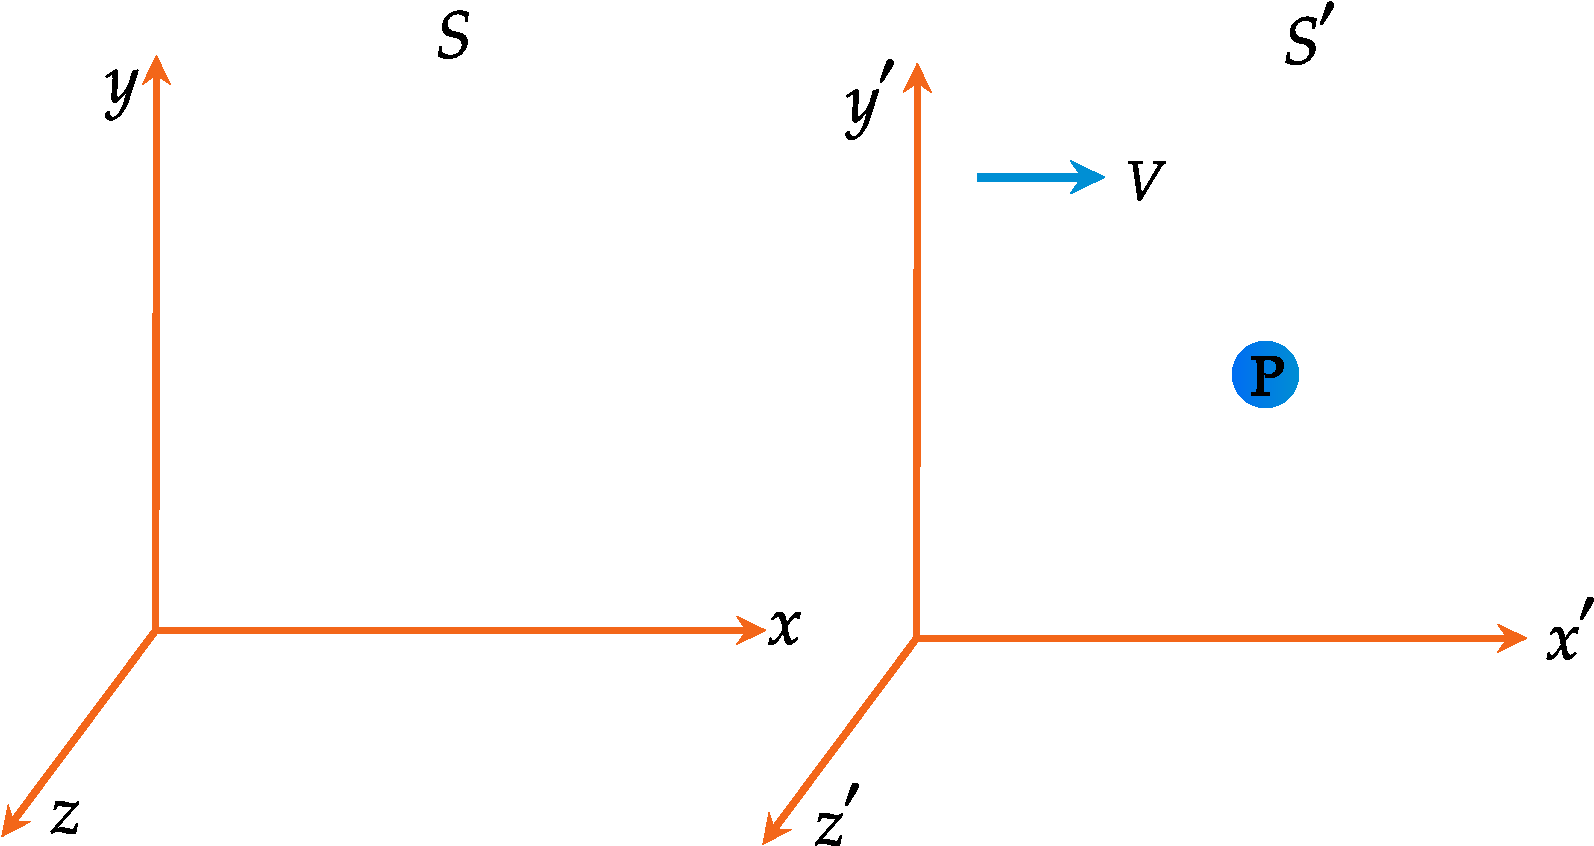
\includegraphics[height=5cm,width=10cm]{lorentz}
	\caption{Lorentz transformation}
	\label{}
\end{figure}
Since the Galilean transformations are inconstitent with some branches of physics we need to replace it with new one. Here we shall derive new equations  using the postulates of special relativity theory and in addition, the assumptio that space and time are homogeneous (All points in space and time are equivalent) \\\\
Our problem can be exactly formulated in the following manner. What are the
values $\mathrm{x}^{\prime}, \mathrm{y}^{\prime}, \mathrm{z}^{\prime}, \mathrm{t}^{\prime}$, of an event with respect to $\mathrm{S}^{\prime}$, when the magnitudes $\mathrm{x}, \mathrm{y}, \mathrm{z}, \mathrm{t}$, of the
same event with respect to $\mathrm{S}$ are given . The relations must be so chosen that the law of the
transmission of light in vacuum is satisfied for one and the same ray of light
 with respect to $\mathrm{S}$ and $\mathrm{S}^{\prime}$. For the relative orientation in space of the co-
ordinate systems , this problem is solved by means of the equations:
\begin{align*}
	x^{\prime} &=\frac{x-v t}{\sqrt{1-\frac{v^{2}}{c^{2}}}} \hspace{2cm} \text{Since,}\ \gamma=\frac{1}{\sqrt{1-v^{2} / c^{2}}} \\
	x^{\prime} &=\gamma ({x-v t})\\
	y^{\prime} &=y \\
	z^{\prime} &=z \\
	t^{\prime} &=\frac{t-\frac{v x}{c^{2}}}{\sqrt{1-\frac{v^{2}}{c^{2}}}}\\
	t^{\prime} &=\gamma ({t-\frac{v x}{c^{2}}})
	\intertext{This system of equations is known as \textbf{Lorentz transformation equations}.}
\end{align*}
\begin{align*}
\intertext{And the inverse transformations are relating $S$\ to \ $S^{\prime}$,}
	x&=\frac{x^{\prime}+v t^{\prime}}{\sqrt{1-v^{2} / c^{2}}} \\
	x&=\gamma (x^{\prime}+v t^{\prime})\\
	y&=y^{\prime} \\
	z&=z^{\prime} \\
	t&=\frac{t^{\prime}+v x^{\prime} / c^{2}}{\sqrt{1-v^{2} / c^{2}}}\\
	t&=\gamma ( t^{\prime}+v x^{\prime} / c^{2})
\end{align*}
\subsection{Velocity transformation}
Thr transformation equations for velocity in Lorentz transformation can be written as,
\begin{align*}
u_{x}^{\prime}&=\frac{u_{x}-v}{1-u_{x} v / c^{2}}\\u_{y}^{\prime}&=\frac{u_{y} \sqrt{1-v^{2} / c^{2}}}{1-u_{x} v / c^{2}}\\
u_{z}^{\prime}&=\frac{u_{z} \sqrt{1-v^{2} / c^{2}}}{1-{u_{x} v / c^{2}}}
\intertext{And the inverse transformations are,}
u_{x}&=\frac{u_{x}^{\prime}+v}{1+u_{x}^{\prime} v / c^{2}}\\
u_{y}&=\frac{u_{y}^{\prime} \sqrt{1-v^{2} / c^{2}}}{1+u_{x}^{\prime} v / c^{2}}\\
u_{z}&=\frac{u_{z}^{\prime} \sqrt{1-v^{2} / c^{2}}}{1+u_{x}^{\prime} v / c^{2}}
\end{align*}
\section{Length contraction}
\begin{figure}[H]
	\centering
	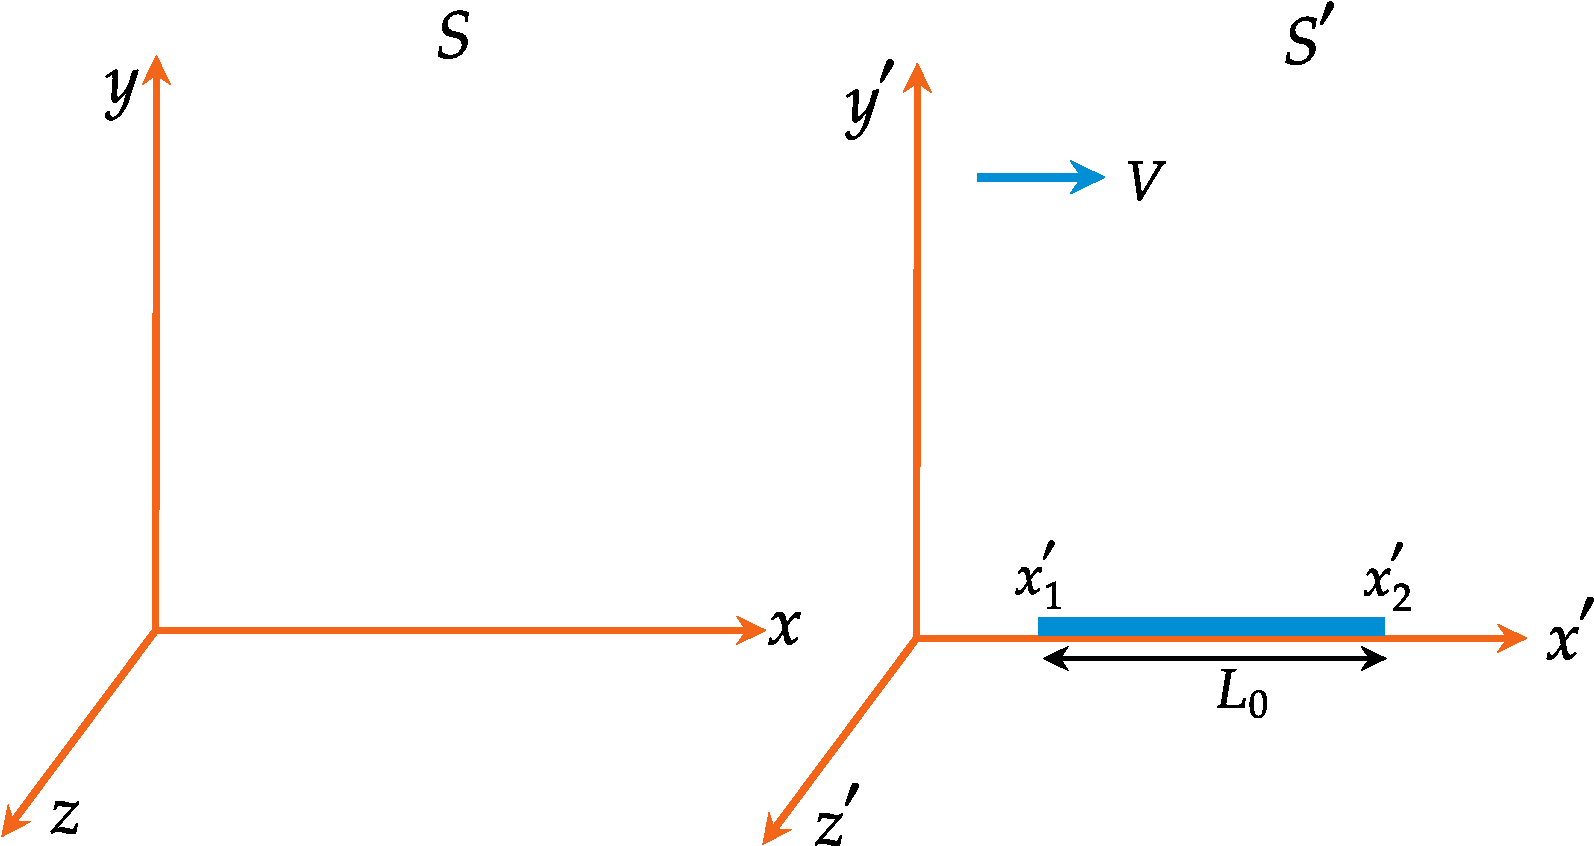
\includegraphics[height=5cm,width=10cm]{length contraction}
	\caption{Length contraction}
	\label{Length contraction}
\end{figure}
If there is a relative motion  between the object and obsever in a system, There will be a discrepancy in measuring it's length .\\
The length $L$ of an object in motion with respect to an observer always appears to the observer to be shorter than it's length $L_{0}$ when it is at rest with respect to the observer. This contraction occurs only in the direction of the relative motion. The length $L_{0}$ of an object in its rest frame is called it's \textbf{proper length}.
\begin{align*}
\intertext { Proper length of rod,} {L}_{0}&=\left({x}_{2}-{x}_{1}\right)\\
\intertext{If $x$ -coordinates of the ends of the rod in reference frame $S^{\prime}$, moving with uniform velocity $v$ with respect to
	frame $\mathrm{S}$ be $\mathrm{x}_{1}^{\prime}$ and $\mathrm{x}_{2}^{\prime}$, as noted simultaneously at same instant $\mathrm{t}^{\prime}$, we have length of rod in moving reference frame $\mathrm{S}^{\prime}$ given by ,}
{L}&=\left({x}_{2}^{\prime}-{x}_{1}^{\prime}\right)
\intertext{According to Lorentz transformation,}
{x}_{1}&=\frac{{{x}_{1}}^{\prime}+{vt}}{\sqrt{1-{v}^{2} / {c}^{2}}} \quad; \quad{x}_{2} =\frac{ {{x}_{2}}^{\prime}+{vt}^{\prime}}{\sqrt{1-{v}^{2} / {c}^{2}}}\\
\text{Then,}\quad L_{0}&=x_{2}-x_{1}\\&=\frac{1}{\sqrt{1-v^{2}  / c^{2}}}\left[x_{2}^{\prime}-x_{1}^{\prime}\right]\\
L_{0}&=\frac{L}{\sqrt{1-v^{2} / c^{2}}}\\
L_{0}&=\gamma L \hspace{2cm} \text{Since,}\ \gamma=\frac{1}{\sqrt{1-v^{2} / c^{2}}}
\end{align*}
\begin{center}
	\framebox{
		\parbox[t][0.8cm]{8cm}{
			
			\addvspace{0.2cm} \centering 
			
			$ L_{0}=\gamma L $ \qquad $\Rightarrow \quad L_{0}=\frac{L}{\sqrt{1-v^{2} / c^{2}}}$} }
\end{center}
\section{Time dilation}
Measurements of time intervals are affected by relative motion between an observer
and what is observed. As a result, a clock that moves with respect to an observer ticks
more slowly than it does without such motion, and all processes  occur more slowly to an observer when they take place in a different inertial frame.\\\\
Let we have two frame of reference, ${S}$ and ${S}^{\prime}$, the former at rest and latter moving with uniform velocity ${v}$, along +ve x-direction.\\
If two events occur at any given point $x$ in frame ${S}^{\prime}$, at time ${t}_{1}^{\prime}$ and $t_{2}^{\prime}$, as noted in the clock carried by it and
at times ${t}_{1}$ and ${t}_{2}$, as noted on the clock carried by frame ${S}$.
\begin{align*}
\intertext{Time interval between two events in frame S,}
\Delta t_{0}&=\left(t_{2}-t_{1}\right)
\intertext{ And we  have time interval between two events, in frame ${S}^{\prime}$}
\Delta t&=\left(t_{2}^{\prime}-t_{1}^{\prime}\right)
\intertext{We have Lorentz transformation equations as, }
t_{1}&=\frac{t_{1}^{\prime}+v_{x}^{\prime} / c^{2}}{\sqrt{1-\frac{v^{2}}{c^{2}}}} \quad ; \quad t_{2}=\frac{t_{2}^{\prime}+v_{x}^{\prime} / t^{2}}{\sqrt{1-v^{2} / c^{2}}}
\intertext{ Then we get the time interval as,}
\Delta t_{0}&=\left(t_{2}-t_{1}\right)\\
&=\frac{t_{2}^{\prime}- t_{1}^{\prime}}{\sqrt{1-v^{2} / c^{2}}}\\&=\frac{\Delta t}{\sqrt{1-v^{2} / c^{2}}}\\
\Delta t_{0}&=\frac{ t_{\text{p}}}{\sqrt{1-v^{2} / c^{2}}}\qquad \Delta t=t_{\text{p}}\\
\Delta t_{0}&=\gamma \ t_{\text{p}}
\end{align*}
Where $t_{\text{p}}$ is the proper time .
\section{Relative velocity}
There is one inertial frame $S, S^{\prime}$ is another inertial frame moving with respect to $S$ in
$x$ -direction and $A$ is another inertial frame which is moving with respect to $S^{\prime}$ with
velocity component $\left(u_{x}^{\prime}, u_{y}^{\prime}, u_{z}^{\prime}\right)$
\begin{align*}
\mathrm{So}, \quad u_{x}^{\prime}&=\frac{d x^{\prime}}{d t^{\prime}} \quad u_{y}^{\prime}=\frac{d y^{\prime}}{d t^{\prime}} \quad u_{z}^{\prime}=\frac{d z^{\prime}}{d t^{\prime}}\\
\intertext{The velocity component of $A$ from $S$ frame is given by,}
u_{x}&=\frac{d x}{d t}, \quad u_{y}=\frac{d y}{d t}, \quad u_{z}=\frac{d z}{d t}
\intertext{ And we  have time interval between two events, in frame ${S}^{\prime}$,}
x&=\gamma\left(x^{\prime}+v t^{\prime}\right), y=y^{\prime}, z=z^{\prime}, t=\gamma\left(t^{\prime}+\frac{v x^{\prime}}{c^{2}}\right)\\\text{Where}\quad \gamma&=\frac{1}{\sqrt{1-\frac{v^{2}}{c^{2}}}}
\intertext { Differentiating both sides, we get ,}
d x&=\gamma\left(d x^{\prime}+v d t^{\prime}\right), \quad d y=d y^{\prime}, \quad d z=d z^{\prime}, \quad d t=\gamma\left(d t^{\prime}+\frac{v d x^{\prime}}{c^{2}}\right)\\
u_{x}&=\frac{d x}{d t}=\gamma\left(\frac{d x^{\prime}+v d t^{\prime}}{d t^{\prime}+\frac{v d x^{\prime}}{c^{2}}}\right)=\frac{\frac{d x^{\prime}}{d t^{\prime}}+v}{1+\frac{v}{c^{2}} \frac{d x^{\prime}}{d t^{\prime}}} \Rightarrow u_{x}=\frac{u_{x}^{\prime}+v}{1+\frac{v}{c^{2}} u_{x}^{\prime}}\\
u_{y}&=\frac{d y}{d t}=\frac{d y^{\prime}}{\gamma\left(d t^{\prime}+\frac{v d x^{\prime}}{c^{2}}\right)}=\frac{\frac{d y^{\prime}}{d t^{\prime}}}{\gamma\left(1+\frac{v}{c^{2}} \frac{d x^{\prime}}{d t^{\prime}}\right)} \quad \Rightarrow u_{y}=\frac{u_{y}^{\prime}}{\gamma\left(1+\frac{v u_{x}^{\prime}}{c^{2}}\right)}\\
u_{z}&=\frac{d z}{d t}=\frac{d z^{\prime}}{\gamma\left(d t^{\prime}+\frac{v d x^{\prime}}{c^{2}}\right)}=\frac{\frac{d z^{\prime}}{d t^{\prime}}}{\gamma\left(1+\frac{v}{c^{2}} \frac{d x^{\prime}}{d t^{\prime}}\right)} \Rightarrow u_{z}=\frac{u_{z}^{\prime}}{\gamma\left(1+\frac{v u_{x}}{c^{2}}\right)}\\
\text { Similarly ,}\quad  u_{x}^{\prime}&=\frac{u_{x}-v}{1-\frac{v u_{x}}{c^{2}}}, \quad u_{y}^{\prime}=\frac{u_{y}}{\gamma\left(1-\frac{v u_{x}}{c^{2}}\right)}, \quad u_{z}^{\prime}=\frac{u_{z}}{\gamma\left(1-\frac{v u_{x}}{c^{2}}\right)}
\end{align*}
\begin{center}
	\framebox{
		\parbox[t][5cm]{4cm}{
			
			\addvspace{0.2cm} \centering 
		\begin{align*}
		u_{x}&=\frac{u_{x}^{\prime}+v}{1+\frac{v}{c^{2}} u_{x}^{\prime}}\\
		u_{y}&=\frac{u_{y}^{\prime}}{\gamma\left(1+\frac{v u_{x}^{\prime}}{c^{2}}\right)}\\
		u_{z}&=\frac{u_{z}^{\prime}}{\gamma\left(1+\frac{v u_{x}}{c^{2}}\right)}
		\end{align*}
			} }
\end{center}
\section{Doppler effect}
\begin{enumerate}
	\item  Observer moving perpendicular to a line between him and the light source. The proper time between ticks is $t_{0}=1 / \nu_{0}$, so between one tick and the next the time $t=t_{0} / \sqrt{1-v^{2} / c^{2}}$ elapses in the reference frame of the observer. The frequency he finds is accordingly
	$$
	\nu(\text { transverse })=\frac{1}{t}=\frac{\sqrt{1-v^{2} / c^{2}}}{t_{0}}
	$$
	Transverse 	doppler effect
	in light
	$$
	\nu=\nu_{0} \sqrt{1-v^{2} / c^{2}}
	$$

	The observed frequency $\nu$ is always lower than the source frequency $\nu_{0}$.\\
	\item  Observer receding from the light source. Now the observer travels the distance $v t$ away from the source between ticks, which means that the light wave from a given tick takes $v t / c$ longer to reach him than the previous one. Hence the total time between the arrival of successive waves is
	$$
	T=t+\frac{v t}{c}=t_{0} \frac{1+v / c}{\sqrt{1-v^{2} / c^{2}}}=t_{0} \frac{\sqrt{1+v / c} \sqrt{1+v / c}}{\sqrt{1+v / c} \sqrt{1-v / c}}=t_{0} \sqrt{\frac{1+v / c}{1-v / c}}
	$$
	and the observed frequency is
	$$
	\nu(\text { receding })=\frac{1}{T}=\frac{1}{t_{0}} \sqrt{\frac{1-v / c}{1+v / c}}=\nu_{0} \sqrt{\frac{1-v / c}{1+v / c}}
	$$
	The observed frequency $\nu$ is lower than the source frequency $\nu_{0}$. Unlike the case of sound waves, which propagate relative to a material medium it makes no difference whether the observer is moving away from the source or the source is moving away from the observer.
	\begin{figure}[H]
		\centering
		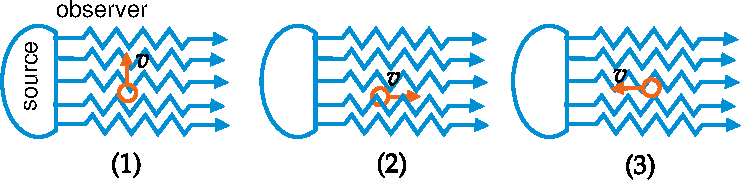
\includegraphics[height=4cm,width=13cm]{Doppler}
		\caption{ The frequency of the light seen by an observer depends on the direction and speed of the observer's motion relative to its source.}
		\label{}
	\end{figure}
	\item  Observer approaching the light source. The observer here travels the distance $v t$ toward the source between ticks, so each light wave takes $v t / c$ less time to arrive than the previous one. In this case $T=t-v t / c$ and the result is
	$$
	\nu(\text { approaching })=\nu_{0} \sqrt{\frac{1+v / c}{1-v / c}}
	$$
	The observed frequency is higher than the source frequency. Again, the same formula holds for motion of the source toward the observer.\\\\
	These two equations can be combined to form a single formula\\
	Longitudinal doppler
	effect in light
	$$
	\nu=\nu_{0} \sqrt{\frac{1+v / c}{1-v / c}}
	$$
	by adopting the convention that $v$ is $+$ for source and observer approaching each other and - for source and observer receding from each other.
\end{enumerate}
\section{ Simultaneity}
An event occurs at $x_{1}$ and $t_{0}$ appears at the time \\
$$
t_{1}^{\prime}=\frac{t_{0}-v x_{1} / c^{2}}{\sqrt{1-v^{2} / c^{2}}}
$$
Next event occurs at  $x_{2}$ and $t_{0}$ appears at the time
$$
t_{2}^{\prime}=\frac{t_{0}-v x_{2} / c^{2}}{\sqrt{1-v^{2} / c^{2}}}
$$
Hence two events that occur simultaneously to one observer are separated by a time interval of\\
$$
t_{2}^{\prime}-t_{1}^{\prime}=\frac{v\left(x_{1}-x_{2}\right) / c^{2}}{\sqrt{1-v^{2} / c^{2}}}
$$
to an observer moving at the speed $v$ relative to the other observer.
\section{Relativistic mass}
The mass of a body moving at the speed v relative to an observer is larger than its mass when at rest relative to the observer by the factor, $\frac{1}{\sqrt{1-\frac{v^{2}}{c^{2}}}}$
\begin{align*}
\text { Thus } \quad m&=\frac{m_{0}}{\sqrt{1-\frac{v^{2}}{c^{2}}}}
\intertext{Where $m_{0}$ is rest mass of body and $\mathrm{m}$ is observed mass.}
\end{align*}
\subsection{Relativistic momentum}
$$
p=m v=\frac{m_{0} v}{\sqrt{1-\frac{v^{2}}{c^{2}}}}
$$
\subsection{Mass and energy}
As we recall from elementary physics, the work $W$ done on an object by a constant force of magnitude F that acts through the distance $s$, where $F$ is in the same direction as $s$, is given by $W=$ Fs. If no other forces act on the object and the object starts from rest, all the work done on it becomes kinetic energy $\mathrm{KE}$, so $\mathrm{KE}=$ Fs. In the general case where F need not be constant, the formula for kinetic energy is the integral
$$
\mathrm{KE}=\int_{0}^{s} F d s
$$
In nonrelativistic physics, the kinetic energy of an object of mass $m$ and speed $v$ is $\mathrm{KE}=\frac{1}{2} \mathrm{~m} v^{2}$. To find the correct relativistic formula for $\mathrm{KE}$ we start from the relativistic form of the second law of motion, which gives
$$\mathrm{KE}=\int_{0}^{s} \frac{d(\gamma m v)}{d t} d s=\int_{0}^{m v} v d(\gamma m v)=\int_{0}^{v} v d\left(\frac{m v}{\sqrt{1-v^{2} / c^{2}}}\right)$$
$\text { Integrating by parts }\left(\int x d y=x y-\int y d x\right) \text {, }$
\begin{align}
	\mathrm{KE} &=\frac{m v^{2}}{\sqrt{1-v^{2} / c^{2}}}-m \int_{0}^{v} \frac{v d v}{\sqrt{1-v^{2} / c^{2}}} \notag \\
	&=\frac{m v^{2}}{\sqrt{1-v^{2} / c^{2}}}+\left[m c^{2} \sqrt{1-v^{2} / c^{2}}\right]_{0}^{v} \notag \\
	&=\frac{m c^{2}}{\sqrt{1-v^{2} / c^{2}}}-m c^{2}\notag\\
	\mathrm{KE}&=\gamma m c^{2}-m c^{2}=(\gamma-1) m c^{2} \label{3.1}
\end{align}
This result states that the kinetic energy of an object is equal to the difference between $\gamma m c^{2}$ and $m c^{2}$. Equation (\ref{3.1}) may be written\\
Total energy
$$
E=\gamma m c^{2}=m c^{2}+\mathrm{KE}
$$
If we interpret $\gamma m c^{2}$ as the total energy $E$ of the object, we see that when it is at rest and $\mathrm{KE}=0$, it nevertheless possesses the energy $m c^{2}$. Accordingly $m c^{2}$ is called the rest energy $E_{0}$ of something whose mass is $m$. We therefore have
$$
E=E_{0}+\mathrm{KE}
$$
 where   
 \begin{equation}
 \text{Rest energy} \quad
 E_{0}=m c^{2} \label{ref3.2}
 \end{equation}
 If the object is moving, its total energy is 
 \begin{equation}
\text{ Total energy} \quad
 E=\gamma m c^{2}=\frac{m c^{2}}{\sqrt{1-v^{2} / c^{2}}}
 \end{equation}
 \begin{figure}[H]
 	\centering
 	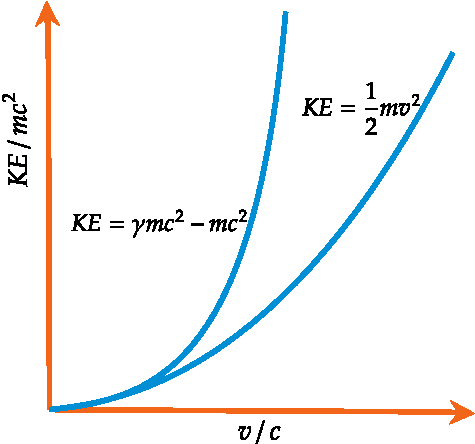
\includegraphics[height=5cm,width=5cm]{str-crop}
 	\caption{ A comparison between the classical and relativistic formulas for the ratio between kinetic energy $\mathrm{KE}$ of a moving body and its rest energy $\mathrm{mc}^{2}$. At low speeds the two formulas give the same result, but they diverge at speeds approaching that of light.}
 	\label{}
 \end{figure}
\begin{exercise}
	A stationary body explodes into two fragments each of mass $1.0 \mathrm{~kg}$ that move apart at speeds of $0.6 c$ relative to the original body. Find the mass of the original body.
\end{exercise}
\begin{answer}
	The rest energy of the original body must equal the sum of the total energies of the fragments. Hence
	$$
	E_{0}=m c^{2}=\gamma m_{1} c^{2}+\gamma m_{2} c^{2}=\frac{m_{1} c^{2}}{\sqrt{1-v_{1}^{2} / c^{2}}}+\frac{m_{2} c^{2}}{\sqrt{1-v_{2}^{2} / c^{2}}}
	$$
	and
	$$
	m=\frac{E_{0}}{c^{2}}=\frac{(2)(1.0 \mathrm{~kg})}{\sqrt{1-(0.60)^{2}}}=2.5 \mathrm{~kg}
	$$
\end{answer}
 \subsection{Energy and Momentum}
 Total energy and momentum are conserved in an isolated system, and the rest energy of a particle is invariant. Hence these quantities are in some sense more fundamental than velocity or kinetic energy, which are neither. Let us look into how the total energy, rest energy, and momentum of a particle are related.
 \begin{align}
  \text { Total energy } \quad
 E&=\frac{m c^{2}}{\sqrt{1-v^{2} / c^{2}}} \label{ref3.4}\\
 \text{ and square it to give} \quad
 E^{2}&=\frac{m^{2} c^{4}}{1-v^{2} / c^{2}}\notag\\
\text{Momentum} \quad p&=\frac{m v}{\sqrt{1-v^{2} / c^{2}}} \label{ref3.5}\\
\text{we find that} \quad p^{2} c^{2}&=\frac{m^{2} v^{2} c^{2}}{1-v^{2} / c^{2}} \notag\\
\text{Now we subtract} \quad p^{2} c^{2}\quad  \text{from} \quad E^{2} \notag \\
E^{2}-p^{2} c^{2} &=\frac{m^{2} c^{4}-m^{2} v^{2} c^{2}}{1-v^{2} / c^{2}}=\frac{m^{2} c^{4}\left(1-v^{2} / c^{2}\right)}{1-v^{2} / c^{2}} \notag \\
&=\left(m c^{2}\right)^{2}\notag\\
\text{Energy and momentum} \quad
E^{2}&=\left(m c^{2}\right)^{2}+p^{2} c^{2} \label{ref3.6}
 \end{align}
  Because $m c^{2}$ is invariant, so is $E^{2}-p^{2} c^{2}$ : this quantity for a particle has the same value in all frames of reference.
\textbf{massless particles}\\
 A particle must have rest mass in order to have energy and momentum, but in relativistic mechanics this requirement does not hold.\\
 From Eqs. (\ref{ref3.4}) and (\ref{ref3.5}), when $m=0$ and $v<< c$, it is clear that $E=p=0$. A massless particle with a speed less than that of light can have neither energy nor momentum. However, when $m=0$ and $v=c, E=0 / 0$ and $p=0 / 0$, which are indeterminate: $E$ and $p$ can have any values. Thus Eqs. (\ref{ref3.4}) and (\ref{ref3.5}) are consistent with the existence of massless particles that possess energy and momentum provided that they travel with the speed of light.
 
 Equation (\ref{ref3.6}) gives us the relationship between $E$ and $p$ for a particle with $m=0$ :\\
 
 Massless particle
 $$E=p c$$
 \begin{exercise}
 	An electron $\left(m=0.511 \mathrm{MeV} / \mathrm{c}^{2}\right)$ and a photon $(m=0)$ both have momenta of $2.000 \mathrm{MeV} / \mathrm{c}$. Find the total energy of each.
 \end{exercise}
\begin{answer}
 (a) the electron's total energy is\\
 \begin{align*}
 	E &=\sqrt{m^{2} c^{4}+p^{2} c^{2}}=\sqrt{\left(0.511 \mathrm{MeV} / c^{2}\right)^{2} c^{4}+(2.000 \mathrm{MeV} / c)^{2} c^{2}} \\
 	&=\sqrt{(0.511 \mathrm{MeV})^{2}+(2.000 \mathrm{MeV})^{2}}=2.064 \mathrm{MeV}
 \end{align*}
 (b) The photon's total energy is\\\\
 $E=p c=(2.000 \mathrm{MeV} / c) c=2.000 \mathrm{MeV}$	
\end{answer}
\section{Space time}
 A length that one observer can measure with only a meter stick may have to be measured with both a meter stick and a clock by another observer. A convenient and elegant way to express the results of special relativity is to regard events as occurring in a four-dimensional spacetime in which the usual three coordinates $x, y, z$ refer to space and a fourth coordinate ict refers to time, where $i=\sqrt{-1}$. Although we cannot visualize spacetime, it is no harder to deal with mathematically than three-dimensional space.
The reason that $i c t$ is chosen as the time coordinate instead of just $t$ is that the quantity
$$
s^{2}=x^{2}+y^{2}+z^{2}-(c t)^{2}
$$
is invariant under a Lorentz transformation. That is, if an event occurs at $x, y, z, t$ in an inertial frame $S$ and at $x^{\prime}, y^{\prime}, z^{\prime}, t^{\prime}$ in another inertial frame $S^{\prime}$, then
$$
s^{2}=x^{2}+y^{2}+z^{2}-(c t)^{2}=x^{\prime 2}+y^{\prime 2}+z^{\prime 2}-\left(c t^{\prime}\right)^{2}
$$
Because $s^{2}$ is invariant, we can think of a Lorentz transformation merely as the orthogonal transformation due to rotation of axes  in spacetime.
\section{Structure of space time}

 The Lorentz transformations take on a simpler appearance when expressed in terms of the quantities
$$
x^{0} \equiv c t, \quad \beta \equiv \frac{v}{c}
$$
Using $x^{0}$ (instead of $t$ ) and $\beta$ (instead of $v$ ) amounts to changing the unit of time from the second to the meter-1 meter of $x^{0}$ corresponds to the time it takes light to travel 1 meter (in vacuum). If, at the same time, we number the $x, y, z$ coordinates, so that
$$x^{1}=x, \quad x^{2}=y, \quad x^{3}=z$$
 then the Lorentz transformations read
 $$\left.\begin{array}{l}
 	\bar{x}^{0}=\gamma\left(x^{0}-\beta x^{1}\right), \\
 	\bar{x}^{1}=\gamma\left(x^{1}-\beta x^{0}\right), \\
 	\bar{x}^{2}=x^{2}, \\
 	\bar{x}^{3}=x^{3} .
 \end{array}\right\}$$
 Or, in matrix form:
 $$\left(\begin{array}{c}
 	\bar{x}^{0} \\
 	\bar{x}^{1} \\
 	\bar{x}^{2} \\
 	\bar{x}^{3}
 \end{array}\right)=\left(\begin{array}{cccc}
 	\gamma & -\gamma \beta & 0 & 0 \\
 	-\gamma \beta & \gamma & 0 & 0 \\
 	0 & 0 & 1 & 0 \\
 	0 & 0 & 0 & 1
 \end{array}\right)\left(\begin{array}{c}
 	x^{0} \\
 	x^{1} \\
 	x^{2} \\
 	x^{3}
 \end{array}\right)$$
 Letting Greek indices run from 0 to 3 , this can be distilled into a single equation:
 $$
 \bar{x}^{\mu}=\sum_{\nu=0}^{3}\left(\Lambda_{\nu}^{\mu}\right) x^{\nu}
 $$
$\text { where } \Lambda \text { is the Lorentz transformation matrix }$\\
\subsection{Four vectors}
 we defined a (3-)vector as any set of three components that transform under rotations the same way $(x, y, z)$ do; by extension, we now define a 4-vector as any set of four components that transform in the same manner as $\left(x^{0}, x^{1}, x^{2}, x^{3}\right)$ under Lorentz transformations:\\
 $$\bar{a}^{\mu}=\sum_{\nu=0}^{3} \Lambda_{\nu}^{\mu} a^{\nu}$$
 For the particular case of a transformation along the x axis, 
$$\begin{aligned}
	&\bar{a}^{0}=\gamma\left(a^{0}-\beta a^{1}\right) \\
	&\bar{a}^{1}=\gamma\left(a^{1}-\beta a^{0}\right) \\
	&\bar{a}^{2}=a^{2} \\
	&\bar{a}^{3}=a^{3}
\end{aligned}$$
\textbf{Scalar product of four vectors}\\
There is a 4-vector analog to the dot product $\left(\mathbf{A} \cdot \mathbf{B} \equiv A_{x} B_{x}+A_{y} B_{y}+A_{z} B_{z}\right)$, but it's not just the sum of the products of like components; rather, the zeroth components have a minus sign:
$$
-a^{0} b^{0}+a^{1} b^{1}+a^{2} b^{2}+a^{3} b^{3} .
$$
 This is the four-dimensional scalar product;\\
 $$
 -\bar{a}^{0} \bar{b}^{0}+\bar{a}^{1} \bar{b}^{1}+\bar{a}^{2} \bar{b}^{2}+\bar{a}^{3} \bar{b}^{3}=-a^{0} b^{0}+a^{1} b^{1}+a^{2} b^{2}+a^{3} b^{3}
 $$
 just as the ordinary dot product is invariant (unchanged) under rotations, this combination is invariant under Lorentz transformations.
To keep track of the minus sign, it is convenient to introduce the covariant vector $a_{\mu}$, which differs from the contravariant $a^{\mu}$ only in the sign of the zeroth component:
$$
a_{\mu}=\left(a_{0}, a_{1}, a_{2}, a_{3}\right) \equiv\left(-a^{0}, a^{1}, a^{2}, a^{3}\right)
$$
 Formally,
 $a_{\mu}=\sum_{\nu=0}^{3} g_{\mu \nu} a^{\nu}, \quad \text { where } \quad g_{\mu \nu} \equiv\left(\begin{array}{rrrr}
 	-1 & 0 & 0 & 0 \\
 	0 & 1 & 0 & 0 \\
 	0 & 0 & 1 & 0 \\
 	0 & 0 & 0 & 1
 \end{array}\right)$
 is the (Minkowski) metric.
The scalar product can now be written with the summation symbol,
$$
\sum_{\mu=0}^{3} a^{\mu} b_{\mu}
$$
or, more compactly still,
$$
a^{\mu} b_{\mu} \text {. }
$$
 Of course, we could just as well take care of the minus sign by switching to covariant $b$ :
$$
a_{\mu} b^{\mu}=a^{\mu} b_{\mu}=-a^{0} b^{0}+a^{1} b^{1}+a^{2} b^{2}+a^{3} b^{3} .
$$
\subsection{Examples of four vectors}
\begin{enumerate}
	\item \textbf{ Position four-vector $ x_{\mu}$}\\
	It is expressed as $x_{\mu}=\left(x_{1}, x_{2}, x_{3}, x_{4}\right)=(\mathbf{r}, i c t)$
	\item \textbf{ Four-velocity or velocity four-vector $u_{\mu}$}\\
	\begin{align*}
		u_{1}&=\frac{d x_{1}}{d \tau}=\frac{d x_{1}}{d t} \frac{d t}{d \tau}=\frac{d x}{d t} \frac{1}{\sqrt{1-u^{2} / c^{2}}}=\frac{u_{x}}{\sqrt{1-u^{2} / c^{2}}} \\
		u_{2}&=\frac{d x_{2}}{d \tau}=\frac{d x_{2}}{d t} \frac{d t}{d \tau}=\frac{d y}{d t} \frac{1}{\sqrt{1-u^{2} / c^{2}}}=\frac{u_{y}}{\sqrt{1-u^{2} / c^{2}}} \\
		u_{3}&=\frac{d x_{3}}{d \tau}=\frac{d x_{3}}{d t} \frac{d t}{d \tau}=\frac{d z}{d t} \frac{1}{\sqrt{1-u^{2} / c^{2}}}=\frac{u_{z}}{\sqrt{1-u^{2} / c^{2}}} \\
		u_{4}&=\frac{d x_{4}}{d \tau}=\frac{d(i c t)}{d t} \frac{d t}{d \tau}=\frac{i c}{\sqrt{1-u^{2} / c^{2}}}\\
		\text{where} \quad \frac{d t}{d \tau}&=\frac{1}{\sqrt{1-u^{2} / c^{2}}}\\
		\text{Hence} \quad u_{\mu}&=\left(u_{1}, u_{2}, u_{3}, u_{4}\right)\\
		or \quad u_{\mu}&=\left(\frac{u_{x}}{\sqrt{1-u^{2} / c^{2}}}, \frac{u_{y}}{\sqrt{1-u^{2} / c^{2}}}, \frac{u_{z}}{\sqrt{1-u^{2} / c^{2}}}, \frac{i c}{\sqrt{1-u^{2} / c^{2}}}\right)\\
		i.e., \quad u_{\mu}&=\left(\frac{\mathbf{u}}{\sqrt{1-u^{2} / c^{2}}}, \frac{i c}{\sqrt{1-u^{2} / c^{2}}}\right)
	\end{align*}
	where $\mathbf{u}=d \mathbf{r} / d t$ is the three dimensional velocity vector.
	The square of the magnitude of the velocity four vector is given by
	$$
	u_{\mu} u_{\mu}=\frac{u^{2}}{1-u^{2} / c^{2}}-\frac{c^{2}}{1-u^{2} / c^{2}}=-c^{2}
	$$
	which is Lorentz invariant.
	\item \textbf{ Momentum four vector $p_{\mu}$}
	\begin{align*}
		&p_{1}=m_{0} u_{1}=\frac{m_{0} u_{x}}{\sqrt{1-u^{2} / c^{2}}}=m u_{x}=p_{x} \\
		&p_{2}=m_{0} u_{2}=\frac{m_{0} u_{y}}{\sqrt{1-u^{2} / c^{2}}}=m u_{y}=p_{y} \\
		&p_{3}=m_{0} u_{3}=\frac{m_{0} u_{z}}{\sqrt{1-u^{2} / c^{2}}}=m u_{z}=p_{z} \\
		&p_{4}=m_{0} u_{4}=\frac{m_{0} i c}{\sqrt{1-u^{2} / c^{2}}}=i m c=i \frac{E}{c}
	\end{align*}
	Hence,
	$$
	p_{\mu}=\left(p_{1}, p_{2}, p_{3}, p_{4}\right)=\left(p_{x}, p_{y}, p_{z}, i m c\right)=(\mathbf{p}, i E / c) \text { with } \mathbf{p}=m \mathbf{u}
	$$
	The square of the magnitude of the four-momentum is given by
	$$
	p_{\mu} p_{\mu}=p^{2}-\frac{E^{2}}{c^{2}}=-\left(E^{2}-p^{2} c^{2}\right) / c^{2} \quad \text { or } \quad p_{\mu} p_{\mu}=-m_{0}^{2} c^{2}
	$$
	This $p_{\mu}$ is also called energy-momentum four-vector.
	\item \textbf{ Acceleration four-vector $a_{\mu}$}\\
	\begin{align*}
	a_{1}&=\frac{d u_{1}}{d \tau}=\frac{d u_{1}}{d t} \frac{d t}{d \tau}=\frac{d}{d t}\left(\frac{u_{x}}{\sqrt{1-u^{2} / c^{2}}}\right) \frac{1}{\sqrt{1-u^{2} / c^{2}}}\\
	&=\frac{1}{\sqrt{1-u^{2} / c^{2}}} \cdot\left(\frac{u_{x}}{\sqrt{1-u^{2} / c^{2}}}+\frac{u_{x} u \dot{u}}{c^{2}\left(1-u^{2} / c^{2}\right)^{3 / 2}}\right)\\
	u^{2}&=u_{x}^{2}+u_{y}^{2}+u_{z}^{2} \text { and hence, } u \dot{u}=u_{x} \dot{u}_{x}+u_{y} \dot{u}_{y}+u_{z} \dot{u}_{z}=\mathbf{u} \cdot \dot{\mathbf{u}}\\
	a_{1}&=\frac{\dot{u}_{x}}{1-u^{2} / c^{2}}+\frac{u_{x}(\mathbf{u} \cdot \dot{\mathbf{u}})}{c^{2}\left(1-u^{2} / c^{2}\right)^{2}}\\
	a_{2}&=\frac{\dot{u}_{y}}{1-u^{2} / c^{2}}+\frac{u_{y}(\mathbf{u} \cdot \dot{\mathbf{u}})}{c^{2}\left(1-u^{2} / c^{2}\right)^{2}}\\
	a_{3}&=\frac{\dot{u}_{z}}{1-u^{2} / c^{2}}+\frac{u_{z}(\mathbf{u} \cdot \dot{\mathbf{u}})}{c^{2}\left(1-u^{2} / c^{2}\right)^{2}}\\
	a_{4}&=\frac{d u_{4}}{d \tau}=\frac{d u_{4}}{d t} \frac{d t}{d \tau}=\frac{d}{d t}\left(\frac{i c}{\sqrt{1-u^{2} / c^{2}}}\right) \frac{1}{\sqrt{1-u^{2} / c^{2}}}=\frac{i(\mathbf{u} \cdot \mathbf{u})}{c\left(1-u^{2} / c^{2}\right)^{2}}\\
	\text { Thus, } \quad a_{\mu}&=\left(\frac{\mathbf{a}}{1-u^{2} / c^{2}}+\frac{\mathbf{u}(\mathbf{u} \cdot \mathbf{a})}{c^{2}\left(1-u^{2} / c^{2}\right)^{2}}, \frac{i(\mathbf{u} \cdot \mathbf{a})}{c\left(1-u^{2} / c^{2}\right)^{2}}\right)\\
\text{where} \mathbf{a}&=\dot{\mathbf{u}}=\dot{u}_{x} \hat{\mathbf{i}}+\dot{u}_{y} \hat{\mathbf{j}}+\dot{u}_{z} \hat{\mathbf{k}}
	\end{align*}
	\item \textbf { Four-force or Minkowski force } $F_{\mu}$\\
	\begin{align}
	F_{\mu}&=\frac{d p_{\mu}}{d \tau}=\frac{d}{d \tau}\left(m_{0} u_{\mu}\right)=m_{0} \frac{d u_{\mu}}{d \tau}=m_{0} \frac{d^{2} x_{\mu}}{d \tau^{2}} \notag\\
	\intertext{This equation is called the Minkowski force equation}
	\intertext{The components of four-force $F_{\mu}$ are}
	F_{1}&=\frac{d p_{1}}{d \tau}=\frac{d p_{1}}{d t} \frac{d t}{d \tau}=\frac{d p_{x}}{d t} \frac{1}{\sqrt{1-u^{2} / c^{2}}}=\frac{F_{x}}{\sqrt{1-u^{2} / c^{2}}}\notag \\
	F_{2}&=\frac{F_{y}}{\sqrt{1-u^{2} / c^{2}}} \notag\\
	F_{3}&=\frac{F_{z}}{\sqrt{1-u^{2} / c^{2}}} \notag\\
	F_{4}&=\frac{d p_{4}}{d \tau}=\frac{d p_{4}}{d t} \frac{d t}{d \tau}=\gamma \frac{d}{d t}\left(\frac{i E}{c}\right)=\frac{i \gamma}{c} \frac{d E}{d t} \notag\\
	F_{\mu}&=\left(\frac{\mathbf{F}}{\sqrt{1-u^{2} / c^{2}}}, \frac{i \gamma}{c} \frac{d E}{d t}\right) \label{ref.str1}\\
	\intertext{The four-force may be expressed in terms of four-acceleration vector as}
	F_{\mu}&=\frac{d p_{\mu}}{d \tau}=\frac{d}{d \tau}\left(m_{0} u_{\mu}\right)=m_{0} \frac{d u_{\mu}}{d \tau}=m_{0} a_{\mu}\notag\\
	F_{\mu}&=\left(\frac{m_{0} \mathbf{a}}{1-u^{2} / c^{2}}+\frac{m_{0} \mathbf{u}(\mathbf{u} \cdot \mathbf{a})}{c^{2}\left(1-u^{2} / c^{2}\right)^{2}}, \frac{i m_{0}(\mathbf{u} \cdot \mathbf{a})}{c\left(1-u^{2} / c^{2}\right)^{2}}\right)\label{ref.str2}\\
	\intertext {Since both equation $\ref{ref.str1}$ and $\ref{ref.str2}$ are the same, equating the space part of $F_{\mu}$,}  \text { we obtain }
	\mathbf{F}&=\frac{m_{0} \mathbf{a}}{\left(1-u^{2} / c^{2}\right)^{1 / 2}}+\frac{m_{0} \mathbf{u}(\mathbf{u} \cdot \mathbf{a})}{c^{2}\left(1-u^{2} / c^{2}\right)^{3 / 2}} \label{ref.str3}\\
	\mathbf{F}&=m \mathbf{a}+\frac{-m \mathbf{u}(\mathbf{u} \cdot \mathbf{a})}{c^{2}-u^{2}} \notag\\
	\intertext { where $\mathbf{F}=d \mathbf{p} / d t$  is the three-dimensional force vector and in general is not equal to $ m \mathbf{a}$} \notag\\
	\text { The fourth component of } &F_{\mu} in \ref{ref.str2} \text { can be written as }\notag \\
	\frac{i m_{0}(\mathbf{u} \cdot \mathbf{a})}{c\left(1-u^{2} / c^{2}\right)^{2}}&=\frac{i \gamma}{c}(\mathbf{F} \cdot \mathbf{u})\label{ref.str4} \\
	\text { because using ($\ref{ref.str3}$) } \notag \\
	\mathbf{F} \cdot \mathbf{u}&=\frac{m_{0}(\mathbf{u} \cdot \mathbf{a})}{\sqrt{1-u^{2} / c^{2}}}+\frac{m_{0}(\mathbf{u} \cdot \mathbf{u})(\mathbf{u} \cdot \mathbf{a})}{c^{2}\left(1-u^{2} / c^{2}\right)^{3 / 2}}=\frac{m_{0}(\mathbf{u} \cdot \mathbf{a})}{\sqrt{1-u^{2} / c^{2}}}\left[1+\frac{u^{2}}{c^{2}-u^{2}}\right] \label{str4}\\
	&=\frac{m_{0}(\mathbf{u} \cdot \mathbf{a})}{\sqrt{1-u^{2} / c^{2}}} \frac{1}{1-u^{2} / c^{2}}=\frac{m_{0}(\mathbf{u} \cdot \mathbf{a})}{\left(1-u^{2} / c^{2}\right)^{3 / 2}} \notag\\
	\intertext { Thus the fourth component of $F_{\mu}$ from ($\ref{ref.str1}$)  and ($\ref{ref.str4}$) is }\\
	\frac{i \gamma}{c} \frac{d E}{d t}&=\frac{i \gamma}{c}(\mathbf{F} \cdot \mathbf{u}) \text { or } \frac{d E}{d t}=\mathbf{F} \cdot \mathbf{u} \label{str5}		
	\end{align}
	The right hand side of eq. ($\ref{str5}$) represents the power and the left hand side for a single particle $d E / d t=d\left(m c^{2}\right) / d t$ represents the rate of change of energy. This is in accordance with the conservation of energy.\\
	Thus the four-force
	$F_{\mu}$ is represented as\\
	\begin{equation}
	F_{\mu}=\left(\frac{\mathbf{F}}{\sqrt{1-u^{2} / c^{2}}}, \frac{i(\mathbf{F} \cdot \mathbf{u})}{c \sqrt{1-u^{2} / c^{2}}}\right)
	\end{equation}
	The Minkowski force equation is
	$F_{\mu}=\frac{d p_{\mu}}{d \tau}=m_{0} \frac{d u_{\mu}}{d \tau}$
\end{enumerate}
\subsection{The space time interval} The scalar product of a 4-vector with itself, $a^{\mu} a_{\mu}=-\left(a^{0}\right)^{2}+\left(a^{1}\right)^{2}+\left(a^{2}\right)^{2}+\left(a^{3}\right)^{2}$, can be positive (if the "spatial" terms dominate) or negative (if the "temporal" term dominates) or zero:\\
If $a^{\mu} a_{\mu}>0, a^{\mu}$ is called spacelike.\\
If $a^{\mu} a_{\mu}<0, a^{\mu}$ is called timelike.\\
If $a^{\mu} a_{\mu}=0, a^{\mu}$ is called lightlike.
\begin{figure}[H]
	\centering
	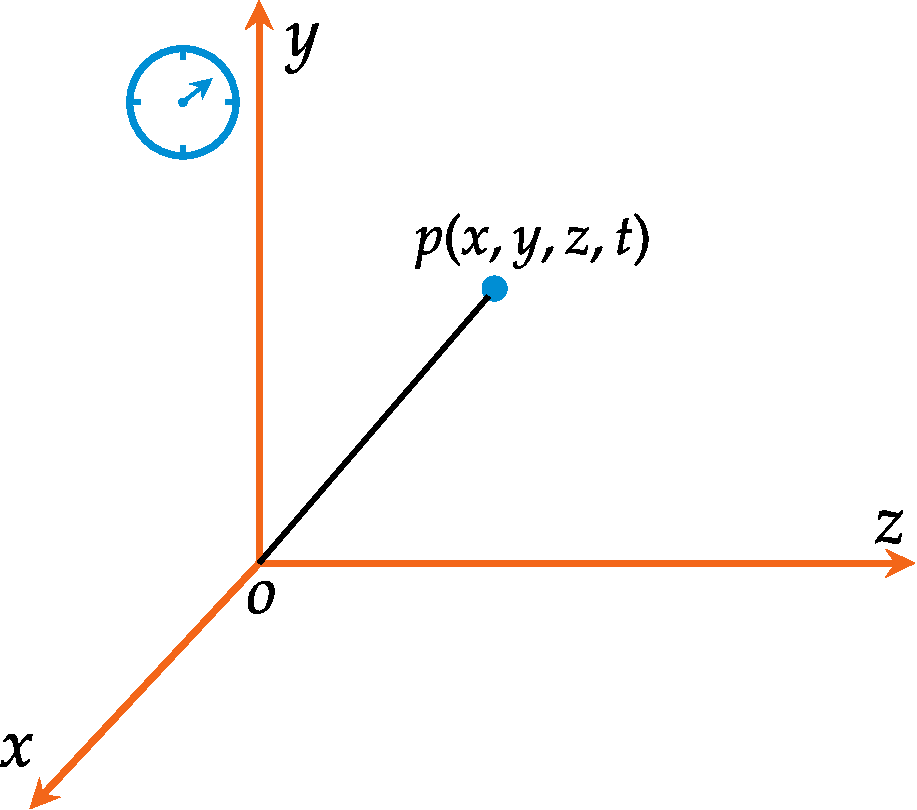
\includegraphics[height=6cm,width=6cm]{str1}
	\caption{}
	\label{fig3.5}
\end{figure}
 Figure $\ref{fig3.5}$ shows two events plotted on the axes $x$ and $c t$. Event 1 occurs at $x=0, t=0$ and event 2 occurs at $x=\Delta x, t=\Delta t$. The spacetime interval $\Delta \mathrm{s}$ between them is defined by\\
 $$\text{ Spacetime interval
 	events}\quad \quad \quad(\Delta s)^{2}=(c \Delta t)^{2}-(\Delta x)^{2}$$
 The virtue of this definition is that $(\Delta s)^{2}$, like the $s^{2}$  is invariant under Lorentz transformations. If $\Delta x$ and $\Delta t$ are the differences in space and time between two events measured in the $S$ frame and $\Delta x^{\prime}$ and $\Delta t^{\prime}$ are the same quantities measured in the $S^{\prime}$ frame,
$$(\Delta s)^{2}=(c \Delta t)^{2}-(\Delta x)^{2}=\left(c \Delta t^{\prime}\right)^{2}-\left(\Delta x^{\prime}\right)^{2}$$
Now let us look into the possible relationships between events 1 and 2 . Event 2 can be related causally in some way to event 1 provided that a signal traveling slower than the speed of light can connect these events, that is, provided that
$$
c \Delta t>|\Delta x|
$$
or
Timelike interval
$$(\Delta s)^{2}>0$$
An interval in which $(\Delta s)^{2}>0$ is said to be timelike. Every timelike interval that connects event 1 with another event lies within the light cones bounded by $x=\pm c t$. All events that could have affected event 1 lie in the past light cone; all events that event 1 is able to affect lie in the future light cone. (Events connected by timelike intervals need not necessarily be related, of course, but it is possible for them to be related.)
Conversely, the criterion for there being no causal relationship between events 1 and 2 is that
$$
c \Delta t<|\Delta x|
$$
or
Spacelike interval
$$(\Delta s)^{2}<0$$
An interval in which $(\Delta s)^{2}<0$ is said to be spacelike. Every event that is connected with event 1 by a spacelike interval lies outside the light cones of event 1 and neither has interacted with event 1 in the past nor is capable of interacting with it in the future; the two events must be entirely unrelated.
When events 1 and 2 can be connected with a light signal only,
$$
c \Delta t=|\Delta x|
$$
or
Lightlike interval
$$
\Delta s=0
$$
An interval in which $\Delta s=0$ is said to be lightlike. Events that can be connected with event 1 by lightlike intervals lie on the boundaries of the light cones.\\
These conclusions hold in terms of the light cones of event 2 because $(\Delta s)^{2}$ is invariant; for example, if event 2 is inside the past light cone of event 1 , event 1 is inside the future light cone of event 2. In general, events that lie in the future of an event as seen in one frame of reference $S$ lie in its future in every other frame $S^{\prime}$, and events that lie in the past of an event in $S$ lie in its past in every other frame $S^{\prime}$. Thus "future" and "past" have invariant meanings.
\begin{figure}[H]
	\centering
	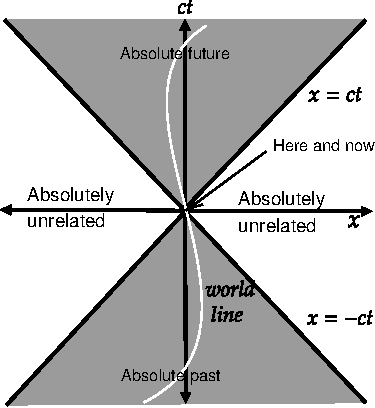
\includegraphics[height=6cm,width=6cm]{str2}
	\caption{The world line of a particle in spae time}
	\label{ref3.6}
\end{figure}
The path of a particle in spacetime is called its world line fig. ($\ref{ref3.6}$). The world line of a particle must lie within its light cones.












\newpage
\begin{abox}
	Practice set 1
	\end{abox}
\begin{enumerate}
	\item Consider the decay process $\tau^{-} \rightarrow \pi^{-}+v_{\tau}$ in the rest frame of the $\tau^{-} .$The masses of the $\tau^{-}, \pi^{-}$and $v_{\tau}$ are $M_{\tau}, M_{\pi}$ and zero respectively.\\
	\textbf{A} The energy of $\pi^{-}$is
	{\exyear{NET JUNE 2011}}
\begin{tasks}(2)
	\task[\textbf{A.}] $\frac{\left(M_{\tau}^{2}-M_{\pi}^{2}\right) c^{2}}{2 M_{\tau}}$
	\task[\textbf{B.}]$\frac{\left(M_{\tau}^{2}+M_{\pi}^{2}\right) c^{2}}{2 M_{\tau}}$
	\task[\textbf{C.}]$\left(M_{\tau}-M_{\pi}\right) c^{2}$
	\task[\textbf{D.}]$\sqrt{M_{\tau} M_{\pi}} c^{2}$
\end{tasks}
\textbf{B} The velocity of  $\pi^{-} \text {is }$
\begin{tasks}(2)
	\task[\textbf{A.}] $\frac{\left(M_{\tau}^{2}-M_{\pi}^{2}\right) c}{M_{\tau}^{2}+M_{\pi}^{2}}$
	\task[\textbf{B.}]$\frac{\left(M_{\tau}^{2}+M_{\pi}^{2}\right) c}{M_{\tau}^{2}-M_{\pi}^{2}}$ 
	\task[\textbf{C.}] $\frac{M_{\pi} c}{M_{\tau}}$
	\task[\textbf{D.}]$\frac{M_{\tau} c}{M_{\pi}}$
\end{tasks}
	\item A constant force $F$ is applied to a relativistic particle of rest mass $m$. If the particle starts from rest at $t=0$, its speed after a time $t$ is
	{\exyear{NET DEC 2011}}

\begin{tasks}(2)
	\task[\textbf{A.}] $\mathrm{Ft} / \mathrm{m}$
	\task[\textbf{B.}]$c \tanh \left(\frac{F t}{m c}\right)$
	\task[\textbf{C.}]$c\left(1-e^{-F t / m c}\right)$
	\task[\textbf{D.}]$\frac{F c t}{\sqrt{F^{2} t^{2}+m^{2} c^{2}}}$
\end{tasks}
	\item Two events separated by a (spatial) distance $9 \times 10^{9} \mathrm{~m}$, are simultaneous in one inertial frame. The time interval between these two events in a frame moving with a constant speed $0.8 c$ (where the speed of light $c=3 \times 10^{8} \mathrm{~m} / \mathrm{s}$ ) is
	{\exyear{NET JUNE 2012}}

\begin{tasks}(2)
	\task[\textbf{A.}] $60 \mathrm{~s}$
	\task[\textbf{B.}]$40 \mathrm{~s}$
	\task[\textbf{C.}]$20 s$
	\task[\textbf{D.}] $0 s$
\end{tasks}
	\item What is proper time interval between the occurrence of two events if in one inertial frame events are separated by $7.5 \times 10^{8} \mathrm{~m}$ and occur $6.5 \mathrm{~s}$ apart?
	{\exyear{NET JUNE 2012}}
\begin{tasks}(2)
	\task[\textbf{A.}] $6.50 \mathrm{~s}$
	\task[\textbf{B.}]$6.00 \mathrm{~s}$
	\task[\textbf{C.}]$5.75 \mathrm{~s}$
	\task[\textbf{D.}]$5.00 \mathrm{~s}$
\end{tasks}
	\item The muon has mass $105 \mathrm{MeV} / \mathrm{c}^{2}$ and mean life time $2.2 \mu \mathrm{s}$ in its rest frame. The mean distance traversed by a muon of energy $315 \mathrm{MeV}$ before decaying is approximately,
{	\exyear{NET DEC 2012}}

\begin{tasks}(2)
	\task[\textbf{A.}] $3 \times 10^{5} \mathrm{~km}$ 
	\task[\textbf{B.}]$2.2 \mathrm{~cm}$
	\task[\textbf{C.}]$6.6 \mu \mathrm{m}$
	\task[\textbf{D.}]$1.98 \mathrm{~km}$
\end{tasks}

	\item The area of a disc in its rest frame $S$ is equal to 1 (in some units). The disc will appear distorted to an observer $O$ moving with a speed $u$ with respect to $S$ along the plane of the disc. The area of the disc measured in the rest frame of the observer $O$ is $(c$ is the speed of light in vacuum)
	{\exyear{NET JUNE 2013}}

\begin{tasks}(2)
	\task[\textbf{A.}] $\left(1-\frac{u^{2}}{c^{2}}\right)^{1 / 2}$
	\task[\textbf{B.}]$\left(1-\frac{u^{2}}{c^{2}}\right)^{-1 / 2}$
	\task[\textbf{C.}]$\left(1-\frac{u^{2}}{c^{2}}\right)$
	\task[\textbf{D.}]$\left(1-\frac{u^{2}}{c^{2}}\right)^{-1}$
\end{tasks}

	\item The recently-discovered Higgs boson at the LHC experiment has a decay mode into a photon and a $Z$ boson. If the rest masses of the Higgs and $Z$ boson are $125 \mathrm{GeV} / \mathrm{c}^{2}$ and $90 \mathrm{GeV} / \mathrm{c}^{2}$ respectively, and the decaying Higgs particle is at rest, the energy of the photon will approximately be
	{\exyear{NET JUNE 2014}}

\begin{tasks}(2)
	\task[\textbf{A.}] $35 \sqrt{3} \mathrm{GeV}$
	\task[\textbf{B.}]$35 \mathrm{GeV}$
	\task[\textbf{C.}]$30 \mathrm{GeV}$
	\task[\textbf{D.}]$15 \mathrm{GeV}$
\end{tasks}
	\item Consider three inertial frames of reference $A, B$ and $C$. the frame $B$ moves with a velocity $\frac{c}{2}$ with respect to $A$, and $C$ moves with a velocity $\frac{c}{10}$ with respect to $B$ in the same direction. The velocity of $C$ as measured in $A$ is
	{\exyear{NET JUNE 2015}}

\begin{tasks}(2)
	\task[\textbf{A.}] $\frac{3 c}{7}$
	\task[\textbf{B.}]$\frac{4 c}{7}$
	\task[\textbf{C.}]$\frac{c}{7}$
	\task[\textbf{D.}] $\frac{\sqrt{3} c}{7}$
\end{tasks}
	\item Consider a particle of mass $m$ moving with a speed $v$. If $T_{R}$ denotes the relativistic kinetic energy and $T_{N}$ its non-relativistic approximation, then the value of $\frac{\left(T_{R}-T_{N}\right)}{T_{R}}$ for $v=0.01 c$, is
	{\exyear{NET DEC 2015}}
\begin{tasks}(2)
	\task[\textbf{A.}] $1.25 \times 10^{-5}$
	\task[\textbf{B.}]$5.0 \times 10^{-5}$
	\task[\textbf{C.}]$7.5 \times 10^{-5}$
	\task[\textbf{D.}]$1.0 \times 10^{-4}$
\end{tasks}
	\item Let $(x, t)$ and $\left(x^{\prime}, t^{\prime}\right)$ be the coordinate systems used by the observers $O$ and $O^{\prime}$, respectively. Observer $O^{\prime}$ moves with a velocity $v=\beta c$ along their common positive $x$ axis. If $x_{+}=x+c t$ and $x_{-}=x-c t$ are the linear combinations of the coordinates, the Lorentz transformation relating $O$ and $O^{\prime}$ takes the form
	{\exyear{NET JUNE 2016}}
\begin{tasks}(2)
	\task[\textbf{A.}] $x_{+}^{\prime}=\frac{x_{-}-\beta x_{+}}{\sqrt{1-\beta^{2}}}$ and $x_{-}^{\prime}=\frac{x_{+}-\beta x_{-}}{\sqrt{1-\beta^{2}}}$
	\task[\textbf{B.}]$x_{+}^{\prime}=\sqrt{\frac{1+\beta}{1-\beta}} x_{+}$and $x_{-}^{\prime}=\sqrt{\frac{1-\beta}{1+\beta}} x_{-}$
	\task[\textbf{C.}]$x_{+}^{\prime}=\frac{x_{+}-\beta x_{-}}{\sqrt{1-\beta^{2}}}$ and $x_{-}^{\prime}=\frac{x_{-}-\beta x_{+}}{\sqrt{1-\beta^{2}}}$
	\task[\textbf{D.}]$x_{+}^{\prime}=\sqrt{\frac{1-\beta}{1+\beta}} x_{+}$and $x_{-}^{\prime}=\sqrt{\frac{1+\beta}{1-\beta}} x_{-}$
\end{tasks}
	\item For a particle of energy $E$ and momentum $p$ (in a frame $F$ ), the rapidity $y$ is defined as $y=\frac{1}{2} \ln \left(\frac{E+p_{3} c}{E-p_{3} c}\right) .$ In a frame $F^{\prime}$ moving with velocity $v=(0,0, \beta c)$ with respect to $F$, the rapidity $y^{\prime}$ will be
	{\exyear{NET JUNE 2016}}
\begin{tasks}(2)
	\task[\textbf{A.}] $y^{\prime}=y+\frac{1}{2} \ln \left(1-\beta^{2}\right)$
	\task[\textbf{B.}]$y^{\prime}=y-\frac{1}{2} \ln \left(\frac{1+\beta}{1-\beta}\right)$
	\task[\textbf{C.}]$y^{\prime}=y+\ln \left(\frac{1+\beta}{1-\beta}\right)$
	\task[\textbf{D.}]$y^{\prime}=y+2 \ln \left(\frac{1+\beta}{1-\beta}\right)$
\end{tasks}
	\item A relativistic particle moves with a constant velocity $v$ with respect to the laboratory frame. In time $\tau$, measured in the rest frame of the particle, the distance that it travels in the laboratory frame is
	{\exyear{NET DEC 2016}}
\begin{tasks}(2)
	\task[\textbf{A.}] $v \tau$
	\task[\textbf{B.}]$\frac{c \tau}{\sqrt{1-\frac{v^{2}}{c^{2}}}}$
	\task[\textbf{C.}]$v \tau \sqrt{1-\frac{v^{2}}{c^{2}}}$
	\task[\textbf{D.}]$\frac{v \tau}{\sqrt{1-\frac{v^{2}}{c^{2}}}}$
\end{tasks}
	\item Consider a radioactive nucleus that is travelling at a speed $\frac{c}{2}$ with respect to the lab frame. It emits $\gamma$-rays of frequency $v_{0}$ in its rest frame. There is a stationary detector, (which is not on the path of the nucleus) in the lab. If a $\gamma$-ray photon is emitted when the nucleus is closest to the detector, its observed frequency at the detector is
	{\exyear{NET DEC 2016}}
\begin{tasks}(2)
	\task[\textbf{A.}] $\frac{\sqrt{3}}{2} v_{0}$
	\task[\textbf{B.}]$\frac{1}{\sqrt{3}} v_{0}$
	\task[\textbf{C.}]$\frac{1}{\sqrt{2}} v_{0}$
	\task[\textbf{D.}]$\sqrt{\frac{2}{3}} v_{0}$
\end{tasks}
	\item An inertial observer sees two events $E_{1}$ and $E_{2}$ happening at the same location but $6 \mu s$ apart in time. Another observer moving with a constant velocity $v$ (with respect to the first one) sees the same events to be $9 \mu s$ apart. The spatial distance between the events, as measured by the second observer, is approximately
{	\exyear{NET JUNE 2017}}
\begin{tasks}(2)
	\task[\textbf{A.}] $300 m$
	\task[\textbf{B.}]$1000 m$
	\task[\textbf{C.}]$2000 m$
	\task[\textbf{D.}]$2700 m$
\end{tasks}
	\item A light signal travels from a point $A$ to a point $B$, both within a glass slab that is moving with uniform velocity (in the same direction as the light) with speed $0.3 c$ with respect to an external observer. If the refractive index of the slab is $1.5$, then the observer will measure the speed of the signal as
	{\exyear{NET DEC 2017}}
\begin{tasks}(2)
	\task[\textbf{A.}] $0.67 c$
	\task[\textbf{B.}]$0.81 c$
	\task[\textbf{C.}]$0.97 c$
	\task[\textbf{D.}] $c$
\end{tasks}
\begin{minipage}{\textwidth}
	\item Two particles $A$ and $B$ move with relativistic velocities of equal magnitude $v$, but in opposite directions, along the $x$-axis of an inertial frame of reference. The magnitude of the velocity of $A$, as seen from the rest frame of $B$, is
	\exyear{NET JUNE 2018}
\end{minipage}
\begin{tasks}(2)
	\task[\textbf{A.}] $\frac{2 v}{\left(1-\frac{v^{2}}{c^{2}}\right)}$ 
	\task[\textbf{B.}]$\frac{2 v}{\left(1+\frac{v^{2}}{c^{2}}\right)}$
	\task[\textbf{C.}] $2 v \sqrt{\frac{c-v}{c+v}}$ 
	\task[\textbf{D.}]$\frac{2 v}{\sqrt{1-\frac{v^{2}}{c^{2}}}}$
\end{tasks}
	\item The energy of a free relativistic particle is $E=\sqrt{|\vec{p}|^{2} c^{2}+m^{2} c^{4}}$, where $m$ is its rest mass, $\vec{p}$ is its momentum and $c$ is the speed of light in vacuum. The ratio $v_{g} / v_{p}$ of the group velocity $v_{g}$ of a quantum mechanical wave packet (describing this particle) to the phase velocity $v_{p}$ is
	{\exyear{NET JUNE 2018}}
\begin{tasks}(2)
	\task[\textbf{A.}] $|\vec{p}| c / E$
	\task[\textbf{B.}]$|\vec{p}| m c^{3} / E^{2}$
	\task[\textbf{C.}] $|\vec{p}|^{2} c^{3} / E^{2}$
	\task[\textbf{D.}]$|\vec{p}| c / 2 E$
\end{tasks}
	\item An inertial frame $K^{\prime}$ moves with a constant speed $v$ with respect to another inertial frame $K$ along their common $x$ - direction. Let $(x, c t)$ and $\left(x^{\prime}, c t^{\prime}\right)$ denote the spacetime coordinates in the frames $K$ and $K^{\prime}$, respectively. Which of the following spacetime diagrams correctly describes the $t^{\prime}$ - axis $\left(x^{\prime}=0\right.$ line $)$ and the $x^{\prime}$ - axis $\left(t^{\prime}=0\right.$ line $)$ in the $x$-ct plane? (In the following figures $\tan \phi=v / c$ )
	{\exyear{NET JUNE 2018}}
\begin{tasks}(2)
	\task[\textbf{A.}]\begin{figure}[H]
		\centering
		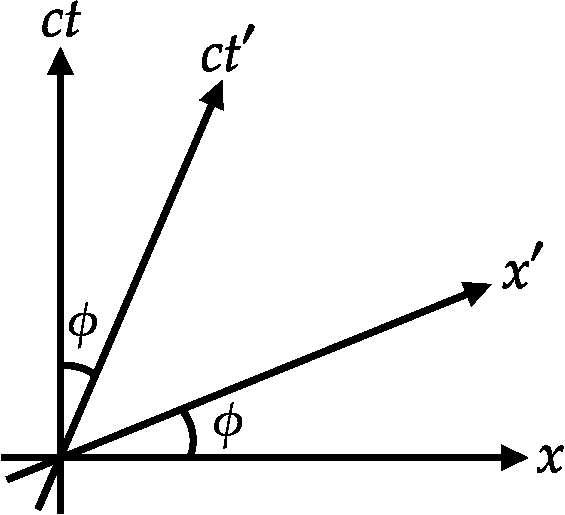
\includegraphics[height=4cm,width=5cm]{PROBLEM 5}
	\end{figure}
	\task[\textbf{B.}]\begin{figure}[H]
		\centering
		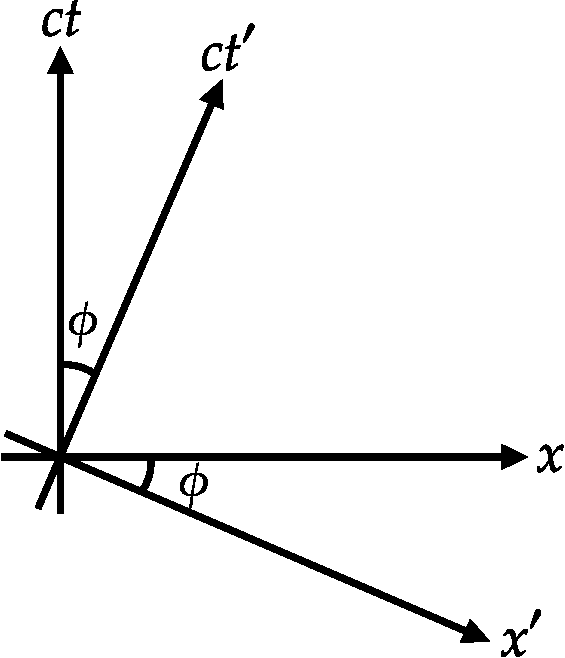
\includegraphics[height=4cm,width=5cm]{PROBLEM 6}
	\end{figure}
	\task[\textbf{C.}]\begin{figure}[H]
		\centering
		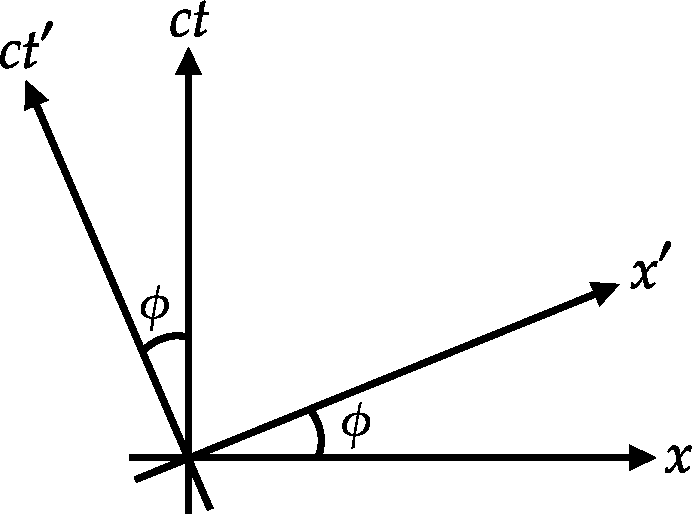
\includegraphics[height=4cm,width=5cm]{PROBLEM 7}
	\end{figure}
	\task[\textbf{D.}]\begin{figure}[H]
		\centering
		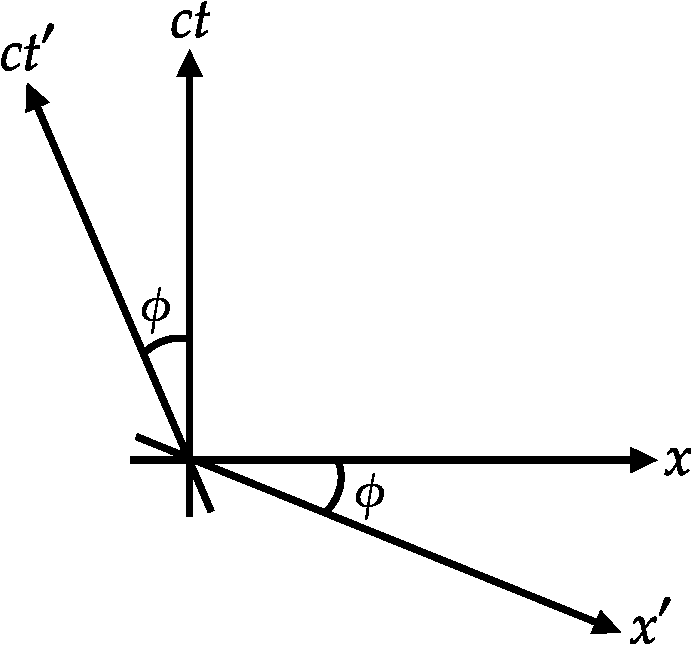
\includegraphics[height=4cm,width=5cm]{PROBLEM8}
	\end{figure}
\end{tasks}
	\item A relativistic particle of mass $m$ and charge $e$ is moving in a uniform electric field of strength $\varepsilon$. Starting from rest at $t=0$, how much time will it take to reach the speed $\frac{c}{2}$ ?
	{\exyear{NET DEC 2018}}
\begin{tasks}(2)
	\task[\textbf{A.}] $\frac{1}{\sqrt{3}} \frac{m c}{e \varepsilon}$
	\task[\textbf{B.}]$\frac{m c}{e \varepsilon}$
	\task[\textbf{C.}]$\sqrt{2} \frac{m c}{e \varepsilon}$
	\task[\textbf{D.}]$\sqrt{\frac{3}{2}} \frac{m c}{e \varepsilon}$
\end{tasks}
\end{enumerate}
\colorlet{ocre1}{ocre!70!}
\colorlet{ocrel}{ocre!30!}
\setlength\arrayrulewidth{1pt}
\begin{table}[H]
	\centering
	\arrayrulecolor{ocre}
	
	\begin{tabular}{|p{1.5cm}|p{1.5cm}||p{1.5cm}|p{1.5cm}|}
		\hline
		\multicolumn{4}{|c|}{\textbf{Answer key}}\\\hline\hline
		\rowcolor{ocrel}Q.No.&Answer&Q.No.&Answer\\\hline
		1&\textbf{A.b,B.a}&2&\textbf{d}\\\hline
		3&\textbf{b}&4&\textbf{b}\\\hline
		5&\textbf{d}&6&\textbf{a}\\\hline
		7&\textbf{c}&8&\textbf{b}\\\hline
		9&\textbf{None}&10&\textbf{d}\\\hline
		11&\textbf{b}&12&\textbf{d}\\\hline
		13&\textbf{a}&14&\textbf{c}\\\hline
		15&\textbf{b}&16&\textbf{b}\\\hline
		17&\textbf{c}&18&\textbf{a}\\\hline
		19&\textbf{a}&&\\\hline
	\end{tabular}
\end{table}
\newpage
\begin{abox}
	Practice set 2
	\end{abox}
\begin{enumerate}
	\item For the set of all Lorentz transformations with velocities along the $x$-axis consider the two statements given below:
	P: If $L$ is a Lorentz transformation, then, $L^{-1}$ is also a Lorentz transformation.
	Q: If $L_{1}$ and $L_{2}$ are Lorentz transformations, then $L_{1} L_{2}$ is necessarily a Lorentz transformation.
	Choose the correct option
{	\exyear{GATE 2010}}
\begin{tasks}(2)
	\task[\textbf{A.}] $P$ is true and $Q$ is false
	\task[\textbf{B.}]Both $P$ and $Q$ are true
	\task[\textbf{C.}]Both $P$ and $Q$ are false
	\task[\textbf{D.}]$P$ is false and $Q$ is true
\end{tasks}
	\item A $\pi^{0}$ meson at rest decays into two photons, which moves along the $x$-axis. They are both detected simultaneously after a time, $t=10 \mathrm{~s} .$ In an inertial frame moving with a velocity $v=0.6 c$ in the direction of one of the photons, the time interval between the two detections is
	{\exyear{GATE 2010}}
\begin{tasks}(2)
	\task[\textbf{A.}] $15 c$
	\task[\textbf{B.}]$0 \mathrm{~s}$
	\task[\textbf{C.}] $10 \mathrm{~s}$
	\task[\textbf{D.}]$20 s$
\end{tasks}	
\begin{minipage}{\textwidth}
	\item Two particles each of rest mass $m$ collide head-on and stick together. Before collision, the speed of each mass was $0.6$ times the speed of light in free space. The mass of the final entity is
	\exyear{GATE 2011}
\end{minipage}
\begin{tasks}(2)
	\task[\textbf{A.}] $5 m / 4$
	\task[\textbf{B.}]$2 m$
	\task[\textbf{C.}]$5 \mathrm{~m} / 2$
	\task[\textbf{D.}]$25 \mathrm{~m} / \mathrm{s}$
\end{tasks}
	\item A rod of proper length $l_{0}$ oriented parallel to the $x$-axis moves with speed $2 c / 3$ along the $x$-axis in the $S$-frame, where $c$ is the speed of light in free space. The observer is also moving along the $x$-axis with speed $c / 2$ with respect to the $S$-frame. The length of the rod as measured by the observer is
	{\exyear{GATE 2012}}
\begin{tasks}(2)
	\task[\textbf{A.}] $0.35 l_{0}$
	\task[\textbf{B.}]$0.48 l_{0}$
	\task[\textbf{C.}]$0.87 l_{0}$
	\task[\textbf{D.}]$0.97 l_{0}$
\end{tasks}
	\item An electron is moving with a velocity of $0.85 c$ in the same direction as that of a moving photon. The relative velocity of the electron with respect to photon is
	{\exyear{GATE 2013}}
\begin{tasks}(2)
	\task[\textbf{A.}] $c$
	\task[\textbf{B.}]$-c$
	\task[\textbf{C.}] $0.15 c$
	\task[\textbf{D.}]$-0.15 c$
\end{tasks}
	\item  The relativistic form of Newton's second law of motion is 
	{\exyear{GATE 2013}}
\begin{tasks}(2)
	\task[\textbf{A.}] $F=\frac{m c}{\sqrt{c^{2}-v^{2}}} \frac{d v}{d t}$ 
	\task[\textbf{B.}]$F=\frac{m \sqrt{c^{2}-v^{2}}}{c} \frac{d v}{d t}$
	\task[\textbf{C.}]$F=\frac{m c^{2}}{c^{2}-v^{2}} \frac{d v}{d t}$
	\task[\textbf{D.}]$F=m \frac{c^{2}-v^{2}}{c^{2}} \frac{d v}{d t}$
\end{tasks}

	\item If the half-life of an elementary particle moving with speed $0.9$ c in the laboratory frame is $5 \times 10^{-8} s$, then the proper half-life is $\times 10^{-8}$ s. $\left(c=3 \times 10^{8} \mathrm{~m} / \mathrm{s}\right)$
	{\exyear{GATE 2014}}
	\item In an inertial frame $S$, two events $A$ and $B$ take place at $\left(c t_{A}=0, \vec{r}_{A}=0\right)$ and $\left(c t_{B}=0, \vec{r}_{B}=2 \hat{y}\right)$, respectively. The times at which these events take place in a frame $S^{\prime}$ moving with a velocity $0.6 c \hat{y}$ with respect to $S$ are given by
	{\exyear{GATE 2015}}

\begin{tasks}(2)
	\task[\textbf{A.}] $c t_{A}^{\prime}=0 ; c t_{B}^{\prime}=-\frac{3}{2}$
	\task[\textbf{B.}]$c t_{A}^{\prime}=0 ; c t_{B}^{\prime}=0$
	\task[\textbf{C.}]$c t_{A}^{\prime}=0 ; c t_{B}^{\prime}=\frac{3}{2}$
	\task[\textbf{D.}] $c t_{A}^{\prime}=0 ; c t_{B}^{\prime}=\frac{1}{2}$
\end{tasks}

	\item A particle with rest mass $M$ is at rest and decays into two particles of equal rest masses $\frac{3}{10} M$ which move along the $z$ axis. Their velocities are given by
	{\exyear{GATE 2015}}
\begin{tasks}(2)
	\task[\textbf{A.}] $\vec{v}_{1}=\vec{v}_{2}=(0.8 c) \hat{z}$
	\task[\textbf{B.}]$\vec{v}_{1}=-\vec{v}_{2}=(0.8 c) \hat{z}$
	\task[\textbf{C.}]$\vec{v}_{1}=-\vec{v}_{2}=(0.6 c) \hat{z}$
	\task[\textbf{D.}]$\vec{v}_{1}=(0.6 c) \hat{z} ; \vec{v}_{2}=(-0.8 c) \hat{z}$
\end{tasks}

	\item The kinetic energy of a particle of rest mass $m_{0}$ is equal to its rest mass energy. Its momentum in units of $m_{0} c$, where $c$ is the speed of light in vacuum, is
	(Give your answer upto two decimal places)
	{\exyear{GATE 2016}}

	\item In an inertial frame of reference $S$, an observer finds two events occurring at the same time at coordinates $x_{1}=0$ and $x_{2}=d$. A different inertial frame $S^{\prime}$ moves with velocity $v$ with respect to $S$ along the positive $x$-axis. An observer in $S^{\prime}$ also notices these two events and finds them to occur at times $t_{1}^{\prime}$ and $t_{2}^{\prime}$ and at positions $x_{1}^{\prime}$ and $x_{2}^{\prime}$ respectively.
	If $\Delta t^{\prime}=t_{2}^{\prime}-t_{1}^{\prime}, \Delta x^{\prime}=x_{2}^{\prime}-x_{1}^{\prime}$ and $\gamma=\frac{1}{\sqrt{1-\frac{v^{2}}{c^{2}}}}$, which of the following statements is true?
	{\exyear{GATE 2016}}
\begin{tasks}(2)
	\task[\textbf{A.}] $\Delta t^{\prime}=0, \Delta x^{\prime}=\gamma d$
	\task[\textbf{B.}] $\Delta t^{\prime}=0, \Delta x^{\prime}=\frac{d}{\gamma}$
	\task[\textbf{C.}]$\Delta t^{\prime}=\frac{-\gamma v d}{c^{2}}, \Delta x^{\prime}=\gamma d$
	\task[\textbf{D.}] $\Delta t^{\prime}=\frac{-\gamma v d}{c^{2}}, \Delta x^{\prime}=\frac{d}{\gamma}$
\end{tasks}

	\item A particle of rest mass $M$ is moving along the positive $x$-direction. It decays into two photons $\gamma_{1}$ and $\gamma_{2}$ as shown in the figure. The energy of $\gamma_{1}$ is $1 \mathrm{GeV}$ and the energy of $\gamma_{2}$ is $0.82 \mathrm{GeV}$. The value of $M$ (in units of $\frac{\mathrm{GeV}}{c^{2}}$ ) is upto two decimal places)
	{\exyear{IIT JAM 201}}
	\begin{figure}[H]
		\centering
		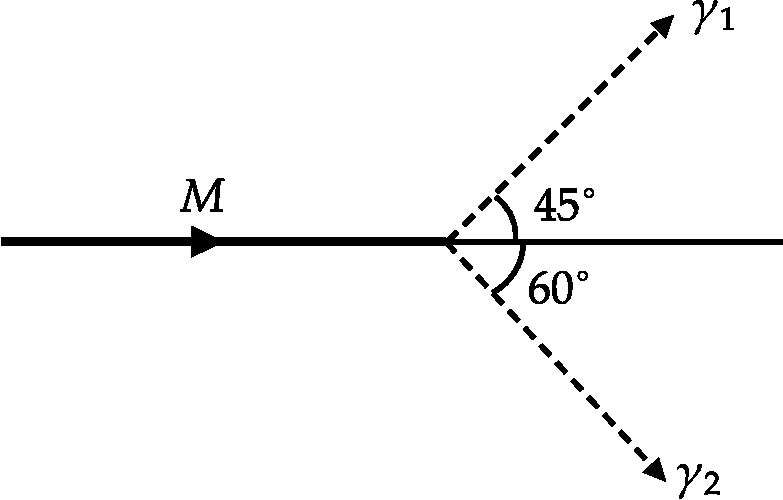
\includegraphics[height=3cm,width=5cm]{problem 17}
	\end{figure}
	\item An object travels along the $x$-direction with velocity $\frac{C}{2}$ in a frame $O$. An observer in a frame $O^{\prime}$ sees the same object travelling with velocity $\frac{C}{4}$. The relative velocity of $O^{\prime}$ with respect to $O$ in units of $c$ is.............. (up to two decimal places).
	{\exyear{GATE 2017}}

	\item A spaceship is travelling with a velocity of $0.7 c$ away from a space station. The spaceship ejects a probe with a velocity $0.59$ c opposite to its own velocity. A person in the space station would see the probe moving at a speed $X_{C}$, where the value of $X$ is (up to three decimal places).
	{\exyear{GATE 2018}}

	\item Two spaceships $A$ and $B$, each of the same rest length $L$, are moving in the same direction with speeds $\frac{4 c}{5}$ and $\frac{3 c}{5}$, respectively, where $c$ is the speed of light. As measured by $B$, the time taken by $A$ to completely overtake $B$ [see figure below] in units of $L / c$ (to the nearest integer) is
	{\exyear{GATE 2019}}$\left. \right. $\\
	\begin{minipage}{0.5\textwidth}
		\begin{figure}[H]
			\centering
			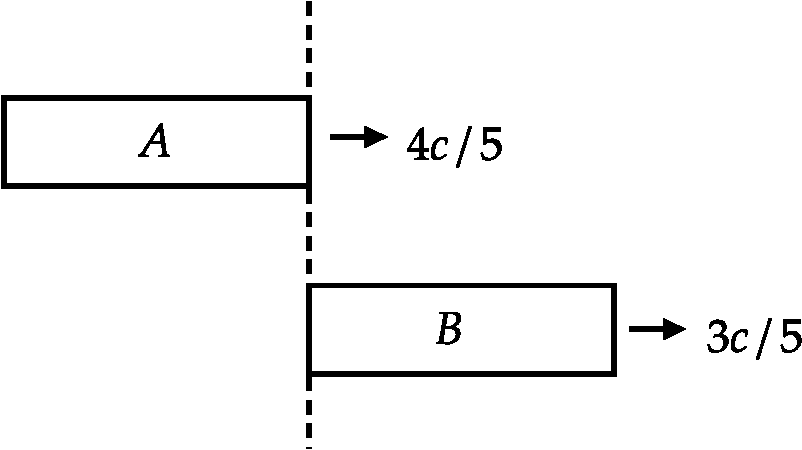
\includegraphics[height=3cm,width=5cm]{PROBLEM 19}
		\end{figure}	
	\end{minipage}
	\begin{minipage}{0.5\textwidth}
		\begin{figure}[H]
			\centering
			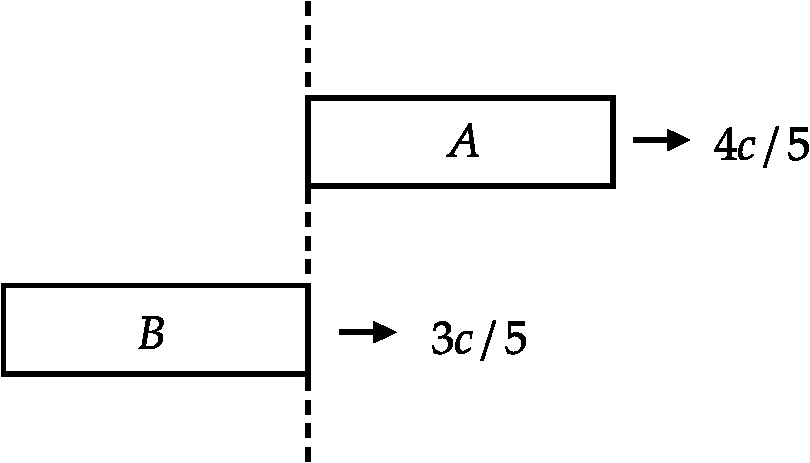
\includegraphics[height=3cm,width=5cm]{PROBLEM 20}
		\end{figure}
	\end{minipage}
	\item Two events, one on the earth and the other one on the Sun, occur simultaneously in the earth's frame. The time difference between the two events as seen by an observer in a spaceship moving with velocity $0.5 c$ in the earth's frame along the line joining the earth to the Sun is $\Delta t$, where $c$ is the speed of light. Given that light travels from the Sun to the earth in $8.3$ minutes in the earth's frame, the value of $|\Delta t|$ in minutes (rounded off to two decimal places) is
	(Take the earth's frame to be inertial and neglect the relative motion between the earth and the sun)
{	\exyear{GATE 2019}}
\end{enumerate}
\colorlet{ocre1}{ocre!70!}
\colorlet{ocrel}{ocre!30!}
\setlength\arrayrulewidth{1pt}
\begin{table}[H]
	\centering
	\arrayrulecolor{ocre}
	
	\begin{tabular}{|p{1.5cm}|p{1.5cm}||p{1.5cm}|p{1.5cm}|}
		\hline
		\multicolumn{4}{|c|}{\textbf{Answer key}}\\\hline\hline
		\rowcolor{ocrel}Q.No.&Answer&Q.No.&Answer\\\hline
		1&\textbf{b}&2&\textbf{a}\\\hline
		3&\textbf{c}&4&\textbf{d}\\\hline
		5&\textbf{b}&6&\textbf{c}\\\hline
		7&\textbf{2.18}&8&\textbf{a}\\\hline
		9&\textbf{b}&10&\textbf{1.732}\\\hline
		11&\textbf{c}&12&\textbf{1.44}\\\hline
		13&\textbf{0.28}&14&\textbf{0.187}\\\hline
		15&\textbf{5}&16&\textbf{4.77}\\\hline
	\end{tabular}
\end{table}

 



























\newpage
\begin{abox}
	Practise Set-3
\end{abox}
\begin{enumerate}[ label=\color{ocre}\textbf{\arabic*.}]

	\item Suppose you are driving your car on a business trip and are traveling at $30 \mathrm{~m} / \mathrm{s}$. Your boss, who is waiting at your destination, expects the trip to take $5.0 \mathrm{~h}$. When you arrive late, your excuse is that your car clock registered the passage of $5.0 $ \ but that you were driving fast and so your clock ran more slowly than your boss's clock. If your car clock actually did indicate a $5.0-\mathrm{h}$ trip, how much time passed on your boss's clock, which was at rest on the Earth?
	\begin{answer}
		\begin{align*}
		\text{	Here, }\quad \gamma&=\frac{1}{\sqrt{1-v^{2} / c^{2}}}=\frac{1}{\sqrt{1-\frac{\left(3 \times 10\  \text{m}/\text{s}^{2}\right)}{\left(3 \times 10^{8} \mathrm{~m} / \mathrm{s}^2\right)}}}\\&=\frac{1}{\sqrt{1-10^{-14}}}
		\intertext{Perform binomial expansion, we get}
		\gamma&=\left(1-10^{-14}\right)^{-1 / 2} \approx 1+\frac{1}{2}\left(10^{-14}\right)=1+\frac{1}{2}\left(10\times 10^{-15}\right) \\&=1+5 \times 10^{-15}
		\intertext{In daily life, $\gamma$ is not much different from $1$.}
		\Delta t&=\gamma \Delta t_{p}\\&=\left(1+5 \times 10^{-15}\right)(5.0 \text{h})=5.0 \text{h}+2.5 \times 10^{-14} \text{h}\\&=5\text{h}+0.09 \mathrm{ns}
		\intertext{Your boss's clock would be only $0.09 \mathrm{~ns}$ ahead of your car clock. }
		\end{align*}
	\end{answer}
	
	\item Imagine a motorcycle moving with a speed $0.80 \mathrm{c}$ past a stationary observer. If the rider tosses a ball in the forward direction with a speed of $0.70 \mathrm{c}$ relative to himself, what is the speed of the ball relativeto the stationary observer?
	\begin{answer}
		\begin{align*}
		\intertext{	The speed of the motorcycle relative to the stationary observer is,} v&=0.8 \mathrm{c}\intertext{The speed of the ball in the frame of reference of the motorcyclist is,}  u_{x}^{\prime}&=0.7 \mathrm{c} . \intertext{Therefore, the speed,$\mathrm{u}_{x}$ of the ball relative to the stationary observer is,}
		u_{x}&=\frac{u_{x}^{\prime}+v}{1+\frac{u_{x}^{\prime} v}{c^{2}}}\\&=\frac{0.70 c+0.80 c}{1+\frac{(0.70  c)(0.80 c)}{c^{2}}}\\&=0.96 c
		\end{align*}
	\end{answer}
	\item An electron, which has a mass of $9.11 \times 10^{31} \mathrm{~kg}$, moves with a speed of $0.750 \mathrm{c}$. Find its relativistic momentum.
	\begin{answer}
		\begin{align*}
		p&=\frac{m_{e} v}{\sqrt{1-\frac{v^{2}}{c^{2}}}}\\
		&=\frac{\left(9.11 \times 10^{-31} \mathrm{~kg}\right)\left(0.750 \times 3.00 \times 10^{8} \mathrm{~m} / \mathrm{s}\right)}{\sqrt{1-\frac{(0\cdot750c)^{2}}{c^{2}}}}\\&=3.10 \times10^{-22} kg\ m/s
		\end{align*}
	\end{answer}
	\item An electron in a television picture tube typically moves with a speed $u=0.25 c$.  Find its total energy and kinetic energy in electron volts.
	\begin{answer}
		\begin{align*}
		\intertext{	Rest energy of electron is $0.511 \mathrm{MeV}$}
		E&=\frac{m_{e} c^{2}}{\sqrt{1-\frac{u^{2}}{c^{2}}}}\\&=\frac{0.511 \mathrm{MeV}}{\sqrt{1-\frac{(0.250 c)^{2}}{c^{2}}}}\\
		&=0.528 \mathrm{MeV}
		\intertext{This is $3 \%$ greater than the rest energy.}
		\intertext{We obtain the kinetic energy by subtracting the rest energy from the total energy:}
		K&=E-m_{e} c^{2}\\&=0.528 \mathrm{MeV}-0.511 \mathrm{MeV}\\&=0.017 \mathrm{MeV}
		\end{align*}
	\end{answer}
	\item (a) Find the rest energy of a proton in electron volts.
	\\(b) If the total energy of a proton is three times its rest energy, with what speed is the proton moving?
	\\(c) Determine the kinetic energy of the proton in electron volts.

	\begin{answer}
		\begin{align*}
		\text{(a)}\quad E_{R}&=m_{p} c^{2}\\&=\left(1.67 \times 10^{-27} \mathrm{~kg}\right)\left(3.00 \times 10^{8} \mathrm{~m} / \mathrm{s}\right)^{2}\\
		&=\left(1.50 \times 10^{-10} J\right)\left(1.00 \mathrm{eV} / 1.60 \times 10^{-19} J\right)\\&=938 \mathrm{MeV}\\\\
		\text{(b)}\quad E&=3 m_{p} c^{2}=\frac{m_{p} c^{2}}{\sqrt{1-\frac{u^{2}}{c^{2}}}} \quad \\3&=\frac{1}{\sqrt{1-\frac{u^{2}}{c^{2}}}}\\
		\text{Solving }&\text{for $'u'$ gives}\\
		1-\frac{u^{2}}{c^{2}}&=\frac{1}{9} \quad \\ \frac{u^{2}}{c^{2}}&=\frac{8}{9}  \\ u&=\frac{\sqrt{3}}{8} c\\&=2.83 \times 10^{8} \mathrm{~m} / \mathrm{s}\\\\
		\text{(c)}\quad K&=E-m_{p} c^{2}\\&=3 m_{p} c^{2}-m_{p} c^{2}=2 m_{p} c^{2}\\
		\text{Because,}\ m_{p} c^{2}&=938 \mathrm{MeV},\\ K&=1.880 \mathrm{MeV}
		\end{align*}
	\end{answer}
	\item A rigid bar of length $1.5 \mathrm{~m}$ is at rest relative to frame $S^{\prime}$. If it makes an angle $\alpha^{\prime}=45^{\circ}$ with $x^{\prime}-$ axis, find the length of the bar and its orientation relative to frame $S$, when $v=0.95 c ?$
	\begin{answer}
		\begin{align*}
		\intertext{Resolving the length of the bar into components parallel to $x^{\prime}$ and $y^{\prime}$ axes, the corresponding length in $S^{\prime}$ are:}
		L_{x}^{\prime}&=L^{\prime} \cos \alpha^{\prime}=1.5 \times 1 / \sqrt{2}=1.06m;\\L_{y}^{\prime}&=L^{\prime}\sin \alpha^\prime-1.5\times1/\sqrt{2}=1.06m
		\intertext{The vertical components would show no contraction, when viewed from $S$ Horizontal component, being parallel to $v$, would}
		\therefore \quad L_{y}&=L_{y}^{\prime}=1.06 m\\
		L_{x}&=L_{x}^{\prime} \sqrt{1-v^{2} / c^{2}}=1.06 \sqrt{1-0.95^{2}}-0.331 m
		\intertext{Therefore, length of the relative $S$ is:}
		L_{1}&=\sqrt{L_{x}^{2}+L_{y}^{2}}=\sqrt{(1.06)+(0.331)}=1.11 \mathrm{~m}\\
		\intertext{	Orientation of the bar relative to $S$ is}
		\tan \alpha&=\frac{L_{y}}{L_{x}}=\frac{1.06}{0.331}=3.20 \quad \\\therefore \alpha&=72^{\circ} 40^{\prime}
		\end{align*}
	\end{answer}
	\item An experimental intends to study a beam of $\pi$ -mesôns of velocity $0.9 c$. How far can he place his apparatus from the target where $\pi$ -measons are produced and still expect to get-sufficient number of $\pi$ -mesons.
	\begin{answer}
		\begin{align*}
		\intertext{ With relativistic time dilation,}
		\Delta t&=\Delta t^{\prime} / \sqrt{1-0.9^{2}}=2.3 \Delta t^{\prime}
		\intertext{Since $\Delta t^{\prime}$ is the time-interval measured by an observer moving with $\pi$ -mesons, it is the real life-time, so that}
		\intertext{$\Delta t^{\prime}=2 \times 10^{-8} s .$ So, in the lab-frame, the mean life is}
		\Delta t&=2.3 \times \Delta t^{\prime}=2.3 \times 2 \times 10^{-8} s\\&=4.6 \times 10^{-8} s
		\intertext{Therefore, average distance travelled by $\pi$ -mesons }&=v . \Delta t=0.9 \times 3 \times 10^{8} \times 4.6 \times 10^{-8} \\\mathrm{~m}&=12.42 \mathrm{~m}
		\end{align*}
	\end{answer}
	\item The half-life of a particular particle as measured in the lab is $4.0 \times 10^{-8} s$ whęn its speed is $0.80 \mathrm{c}$ and $3 \times 10^{-8} s$ when its speed is $0.60 \mathrm{c}$. Find its actual life time.
	\begin{answer}
		\begin{align*}
		\intertext{Due to time-dilation, the half-life of a moving particle appears lengthened. Let $\Delta t_{0}$ be the actual half-life, i.e.,in the frame of reference of the particle, and $\Delta t$ that measured by a stationary observer.}
		\therefore \quad \Delta t&=\Delta t_{0} / \sqrt{1-v^{2} / c^{2}}\\
		\intertext{Therefore, by the problem}
		4.0 \times 10^{-8}&=\frac{\Delta t}{\sqrt{1-0.8^{2}}} ; 3.0 \times 10^{-8}=\frac{\Delta t_{0}}{\sqrt{1-0.6^{2}}}
		\intertext{Either relation gives, $\Delta t_{0}=2.4 \times 10^{-8} s$, the actual life-time.}
		\end{align*}
	\end{answer}
	\item What will be the period of the 'seconds' pendulum measured by an observer moving with a speed of $0.8 \mathrm{c}$ ?
	\begin{answer}
		\begin{align*}
		\intertext{If $T_{0}(=2 s)$ be the period of a seconds pendulum asmeasured by an observer at rest, the same would be, say To the moving observer}
		\intertext{Therefore, from the time-dilation relation,}
		T&=\frac{T_{0}}{\sqrt{1-v^{2} / c^{2}}}=\frac{2}{\sqrt{1-0.8^{2}}}=3.33 s
		\end{align*}
	\end{answer}
	\item The average life-time of neutron is $5$min. It disintegrates spontaneously in to an electron,a proton and a neutrino. Ifthe distance of the sun from the earth is $11 \times 10^{10} m_{i}$ find the average minimum velocity with which a neutron must leave the sun so.as to reach the earth before breaking up.
	\begin{answer}
		\begin{align*}
		\intertext{Let $v$ be the required velocity of the neutron. The time $t_{1}$ for neutron to reach the earth from the sun before decay is}
		t_{1}&=\frac{11 \times 10^{10} m}{v}\\
		\intertext{If $t_{0}$ be the life-time of neutron at rest, then the average life-time $t$ of the 'moving' neutro, as measured by an observer on earth, is}
		t&=\frac{t_{0}}{\sqrt{1-v^{2} / c^{2}}}=\frac{15 \times 60 s}{\sqrt{1-v^{2} / c^{2}}}
		\intertext{Plainly, this $t$ and previous $t_{1}$ must be equal,}
		\therefore \quad \frac{11 \times 10^{10}}{v}&=\frac{15 \times 60}{\sqrt{1-v^{2} /\left(3 \times 10^{8}\right)^{2}}}
		\intertext{Simplifying, we obtain,}
		v&=1.132 \times 10^{8} \mathrm{~ms}^{-1}
		\end{align*}
	\end{answer}
	\item A rocket is travelling towards the moon with a velocity $0.6 \mathrm{c}$. When half-way to the moon, it fires a message rocket back towards the earth with a velocity $0.8 \mathrm{c}$ relative to the primary rocket. What a velocity of the message rocket as seen by a terrestrial observer? Neglect the recoil.
	\begin{answer}
		\begin{align*}
		\intertext{The velocity of the message rocket relative to a terrestrial observer is, by velocity addition theorem,}
		v&=\frac{(0.6-0.8) c}{1-0.8 \times 0.6}=\frac{-0.2 c}{1-0.48}\\
		&=-\frac{0.2 c}{0.52}\\&=-0.385 c
		\intertext{The negative sign indicates that the rocket is moving towards the earth.}
		\end{align*}
	\end{answer}

\item \texttt{ How many years does it take for an atomic clock (with a precision of one part over} $10^{15}$ ), which is placed at rest on Earth, to lose one second with respect to an identical clock placed on the Sun? (Hint: apply Lorentz transformations as if both reference frames were inertial, with a relative velocity $v \simeq 310^{4} \mathrm{~m} / \mathrm{s} \simeq 10^{-4} \mathrm{c}$ ).
\begin{answer}
	\begin{align*}
	\text{Setting,}\ \Delta t&=1s\\ \text{We have,}\ T&=\frac{\Delta t}{\left(1-\sqrt{1-v^{2} / c^{2}}\right)} \\& \simeq 2 \Delta t \frac{c^{2}}{v^{2}}\\& \simeq 6.34 \text{years.}
	\end{align*}
\end{answer}
\end{enumerate}
{\fontfamily{qcr}\selectfont
	which is placed at rest on Earth.
}\\
{\fontfamily{lmdh}\selectfont
	which is placed at rest on Earth.
}\\
{\fontfamily{cmr}\selectfont
	which is placed at rest on Earth.
}



